\documentclass[dvipdfmx]{jsreport}


\usepackage[letterpaper,top=2cm,bottom=2cm,left=3cm,right=3cm,marginparwidth=1.75cm]{geometry}

\usepackage{amsmath}
\usepackage{graphicx}
\usepackage[colorlinks=true, allcolors=blue]{hyperref}

\begin{document}

\begin{titlepage}
   \begin{center}
       \vspace*{2cm}

       \huge
       令和4年度卒業論文\\
       \vspace{0.5cm}
       \textbf{Rydberg状態励起用レーザーの開発と\\電磁誘起透明化信号の観測}
       
       \vspace{0.5cm}
       \LARGE
        Development of lasers for excitation of Rydberg states and observation of electromagnetically induced transparency signal

       \large
       \vspace{2cm}
       応用理工系学科 応用物理工学コース \\
       
       \vspace{1cm}
       フォトニクス研究室 \\
       
    \vspace{1cm}
       佐藤一徹 \\
            
       \vspace{1cm}
       2023年2月7日            
   \end{center}
\end{titlepage}

\setcounter{tocdepth}{3}
\tableofcontents

\clearpage
\chapter{序論}
\section{研究背景}
\subsection{レーザー冷却}
レーザー冷却技術の発展は、量子力学レベルでの原子の制御を可能にし、極低温における物理を進展させている。1995年にはアインシュタインによって予言されていた極低温現象であるボース・アインシュタイン凝縮(BEC)が観測され、2001年のノーベル物理学賞の対象となった。\cite{bose}極低温で観測される原子間の新たな弱い結合メカニズムは科学の一分野として注目されており、Feshbach共鳴\cite{fesh}、Efimov状態\cite{efimov}などに加え、極低温分子の生成・応用も進んでいる。例えば、2019年には極低温分子を用いた精密分光による電子と陽子の質量比の恒常性実験が行われ、精度がそれまでの5倍程更新された。\cite{kobayashi}本研究室ではRb原子を用いた研究を立ち上げており、昨年は光格子と呼ばれるレーザー光の定在波から形成される周期的なポテンシャル中に原子をトラップし、ラマンサイドバンド冷却と圧縮を繰り返すことで高速なBECの実現を目指す実験が行われた。\cite{okuda}効率的で高速なBECの実現、そこから極低温分子の生成、精密分光実験を目指している。

\subsection{Rydberg原子}
以上のような極低温現象の探究と並行して、Rydberg原子もまた、レーザー冷却の応用として注目されている。Rydberg原子は、Rydberg状態と呼ばれる価電子が高い主量子数状態(通常、$n=10\sim200$程度)に励起された、軌道半径が大きい中性原子である。最外殻電子は基底状態の原子と比較して$100\sim1000$倍も原子の中心から離れているため、分極性が向上している\cite{rydberg}。これはまた、誘導双極子モーメントの増加や強い長距離双極子-双極子相互作用にもつながる。

Rydberg原子の顕著な特徴の一つに、Rydberg blockadeと呼ばれる効果がある。これは、隣接するRydberg原子との相互作用により、原子のRydberg準位がレーザーに対して共鳴しないようにシフトされ、一定の体積中でRydberg励起される原子は一つだけになるという現象である。Rydberg blockadeは、レーザーによる冷却・トラップ技術と併せて量子コンピュータの実現に向けた研究などに応用されている。\cite{yuma}

また、イオンとRydberg原子間の新たな分子結合\cite{ion-rydberg}や、数十mV/cm程度の電場によってRydberg原子がイオン化されること(field ionization)を利用したRydberg分光\cite{yuma}など、我々の研究室のテーマである極低温分子の生成、精密分光とも相性の良い分野であると言える。
\section{目的}
本研究室ではRydberg原子を、field ionizaitonを利用した原子の高感度検出に利用することを考えている。field ionizationに必要な電場は、
\begin{equation}
    F_{\text{ioniz.}} = \frac{F_0}{16 {n^*}^4}
\end{equation}
と表せる。\cite{rucas}ここで、$F_0$は電場の原子単位で$F_0 \simeq 5 \times 10^9$V/cmであり、$n^*$は後に説明する実行主量子数と呼ばれる量である。例えば、実験室で使える電場が100V/cmだとすると、イオン化に必要な条件は$n^* \geq 42.04482$である。

本研究では、Rb原子をRydberg励起するためのレーザーシステムの開発を目的とした。周波数調整可能な光源を2種類用意し、一方を基底状態から中間状態への励起、もう一方を中間状態からRydberg状態への励起に使用する。これらのレーザーの周波数を、原子の共鳴周波数や理論によって求める値に安定化させることで、別の実験系にRydberg励起用の光を提供できるようにする。また、実際にRydberg励起が起きていることを本システムの中で確認できるようにするために、三準位系と光の相互作用に特有の現象である電磁誘起透明化信号を観測できるようにする。さらに、電磁誘起透明化信号が観測できる範囲で、可能な限り大きな主量子数へのRydberg励起を目指した。

\clearpage
\chapter{原理}
\section{Rydberg励起に必要なレーザー}
\label{sec:rydberg}
Rydberg準位に原子を励起するために、適切な波長(周波数)のレーザーを用意する必要がある。水素原子のエネルギー準位(ポテンシャルエネルギー)は、非相対論的近似において、
\begin{equation}
\label{rydberg}
 E_n = -hc\frac{R_{\infty}}{n^2},\; \left(R_{\infty} = \frac{m_e e^4}{8 \epsilon_0^2 h^3 c} \right)
\end{equation}

\begin{equation}
 k = \frac{1}{\lambda} = R_{\infty}\left( \frac{1}{{n_1^*}^2} - \frac{1}{{n_2^*}^2} \right)
\end{equation}

で表される。ここで$R_{\infty}$はRydberg定数、$m_e$は電子質量、$e$は電子の電荷、$\epsilon_0$は真空の誘電率、$h$はプランク定数である。RbのRydberg原子の場合、エネルギー準位は量子欠損による補正を受けて
\begin{equation}
 E_{n,l,j} = -hc\frac{R_{Rb}}{{n^*}^2},\; \left( R_{Rb} = \frac{R_{\infty}}{1 + m_e / m_c} \right)
\end{equation}
となる。ここで$m_c$は原子核質量、$R_{Rb}$はRbの電子質量が減少した時のRydberg定数で$R_{Rb} \simeq 109,736.605\text{cm}^{-1}$、${n^*} = n - \delta_{n,l,j}$は実効主量子数である。$\delta_{n,l,j}$は量子欠損と呼ばれ、Rydberg原子が原子核付近に近づいた時に生じる、他の電子からの多体的な効果を現象論的に補正するための量である。量子欠損の値は、$n > 20$程の大きな主量子数において近似的に
\begin{equation}
\delta_{n,l,j} = \delta_0(l,j) + \frac{\delta_2(l,j)}{n - \delta_0(l,j)}
\end{equation}
と表せる。$\delta_n$はRydberg準位の分光結果をフィッティングすることで求められる。本実験では、表\ref{table:qd}に示す、先行研究\cite{quantum-defect}(Millimeter-wave spectroscopy of cold Rb Rydberg atoms in a magneto-optical trap: Quantum defects of the ns, np, and nd series)で測定された量子欠損の値を用いた。
\begin{table}[hbtp]
  \caption{s,p,d軌道の量子欠損パラメータ}
  \label{table:qd}
  \centering
  \begin{tabular}{lll}
    \hline
    電子配置  & $\delta$ & 波数(誤差)[cm$^-1$] \\
    \hline
    \hline
    $nS_{1/2}$  & $\delta_0$ & 3.1311804(10) \\
                        & $\delta_2$ & 0.1784(6) \\
    $nP_{1/2}$  & $\delta_0$ & 2.6548849(10) \\
                        & $\delta_2$ & 0.2900(6) \\
    $nP_{3/2}$  & $\delta_0$ & 2.6416737(10) \\
                     & $\delta_2$ & 0.2950(7) \\
    $nD_{3/2}$  & $\delta_0$ & 1.34809171(40) \\
                        & $\delta_2$ & -0.60286(26) \\
    $nD_{5/2}$  & $\delta_0$ & 1.34646572(30) \\
                        & $\delta_2$ & -0.59600(18) \\
    \hline
  \end{tabular}
\end{table}

今、二つの準位間(特に基底状態である$5S_{1/2}$から中間準位である$6P_{3/2}$、及び$6P_{3/2}$からRydberg準位)の遷移に必要な周波数を求めたいが、$5S_{1/2}$や$6P_{3/2}$のエネルギー準位は量子欠損を含めた計算だと合わないので文献値\cite{nist}(NIST Atomic Spectra Database Levels Data)を参照する。計算に使用した値を表\ref{table:nist}に示す。
\begin{table}[hbtp]
  \caption{基底状態からの励起に必要なレーザーの波数 \\
  NIST Atomic Spectra Database Levels Data\cite{nist}より抜粋}
  \label{table:nist}
  \centering
  \begin{tabular}{lll}
    \hline
    電子配置  & 波数[cm$^-1$] & 誤差 \\
    \hline
    \hline
    $5S_{1/2}$ & 0.000 & 0.010 \\
    $6P_{3/2}$ & 23792.591 & 0.010 \\
    Limit & 33690.81 & 0.010 \\
    \hline
  \end{tabular}
\end{table}

荷電子を$5S_{1/2}$から準位エネルギーがゼロの状態に励起(=イオン化)するのに必要な波数は$k_{\text{lim}} = 33690.81 \pm 0.01\text{cm}^{-1}$、$5S_{1/2}$から$6P_{3/2}$に励起するのに必要な波数は$k_{\text{6P}} = 23792.591 \pm 0.010\text{cm}^{-1}$である。準位エネルギーは$E_n = -hk_nc$と表せるから、$5S_{1/2}$から任意の状態への励起に相当する波数$k_e$は、
\begin{align}
\begin{split}
\label{rydberg-frequency}
k_e &= k_{\text{lim}} - k_n \\
&= k_{\text{lim}} - \frac{R_{Rb}}{{n^*}^2}
\end{split}
\end{align}
と表せる。$6P_{3/2}$から任意の準位への励起に相当する波数は、さらに$k_e^{'} = k_e - k_{\text{6P}}$を計算すれば良い。波数$k$が求められれば、周波数は$\omega = ck$、波長は$\lambda = 1 / k$と簡単に求めることができる。

本実験では、二つの外部共振器型半導体レーザー(ECDL)を用いて、中間準位$6P_{3/2}$を経由したRydberg励起を目指した。ここまでの式より、$5S_{1/2}$から$6P_{3/2}$への励起に必要な波長は$420.2989073(\pm 1766)\text{nm}\; \left(= 713.2839338(\pm 2998)\text{THz} \right)$、$6P_{3/2}$から$30D_{5/2}$への励起に必要な波長は$1024.091256(\pm 2104)\text{nm}\; \left(= 292.739984(\pm 6012)\text{THz} \right)$である。したがって、本論文では中間準位への励起に用いた波長420nm付近のレーザーをECDL1、Rydberg状態への励起に用いた波長1024nm付近のレーザーをECDL2と呼ぶ。

\clearpage
\section{飽和吸収分光(Saturated Absorption Spectroscopy)}
ここでは、ECDL1をRbの共鳴周波数に安定化するために用いた、飽和吸収分光とその応用である変調移行分光の原理を説明する。
\subsection{ドップラー吸収}
レーザー光が進む方向を$x$軸とする。$x$方向に速度$v$で運動する原子から見ると、レーザー周波数$\omega$はドップラー効果によって次のように変化する。

\begin{equation}
\omega' = \omega - kv
\end{equation}

ここで、$k = \omega / c = 2\pi / \lambda$である。すなわち、速度$v$で運動する原子は、原子の共鳴周波数を$\omega_0$とすると、$\delta = \omega - \omega_0 = kv$の時、共鳴する。これは、
\begin{equation}
\label{doppler}
    \frac{\delta}{\omega_0} = \frac{v}{c}
\end{equation}
と等価である。室温において気体原子は熱運動しており、速度$v$から$v + dv$の範囲に原子が分布している割合は次のように表せる。

\begin{equation}
    f(v)dv 
    = \sqrt{\frac{M}{\pi2k_BT}}\text{exp}\left( - \frac{Mv^2}{2k_BT} \right)dv
    \equiv \frac{1}{u\sqrt{\pi}}\text{exp} \left( - \frac{v^2}{u^2} \right)dv
\end{equation}

ここで、$u=\sqrt{2k_BT/M}$、$M$は原子の質量、$T$は温度である。式(\ref{doppler})より速度を周波数に変換すると、光の吸収スペクトルは速度分布を反映したガウス分布となる。

\begin{equation}
    g_D(\omega) = 
    \frac{c}{u\omega_0\sqrt{\pi}}
    \text{exp}
    \left\{
        -\frac{c^2}{u^2}
        \left(
            \frac{\omega - \omega_0}{\omega_0}
        \right) ^2
    \right\}
\end{equation}

この分布の半値全幅$\Delta\omega_D$は次のように与えられる。

\begin{equation}
\frac{\Delta\omega_D}{\omega_0} = 2\sqrt{\log2}u/c \simeq 1.7u/c
\end{equation}

$u$は速度分布の中央の速度であり、原子の質量と温度に依存する。Rbの時、$\Delta\omega_D/\omega_0 = 1.37\times10^{-5}$程度である。すなわち、半値全幅$\Delta\omega_D\simeq\text{9.78GHz}$である。詳細な導出は\cite{foot}を参照されたい。超微細構造によるスペクトルの分岐は数十MHzから数GHz程度であるため、ドップラー幅に埋もれてしまう。これを回避する手段の一つが、飽和吸収分光である。

\subsection{飽和吸収分光}
\begin{figure}
\centering
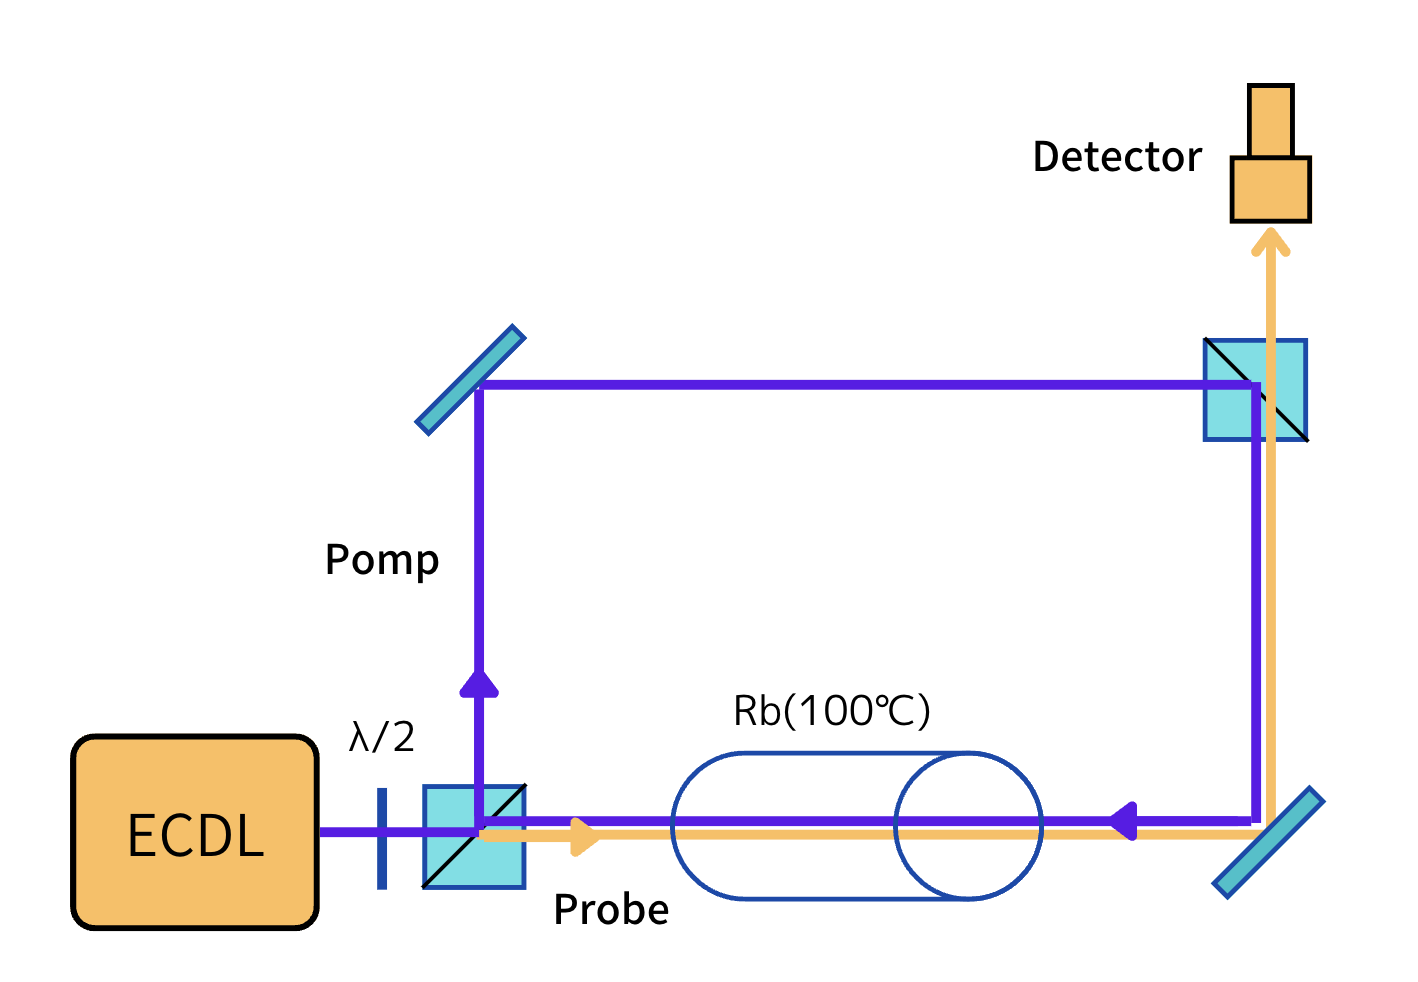
\includegraphics[width=0.6\textwidth]{images/sas.png}
\caption{\label{fig:sas}飽和吸収分光の概要}
\end{figure}
\begin{figure}
\centering
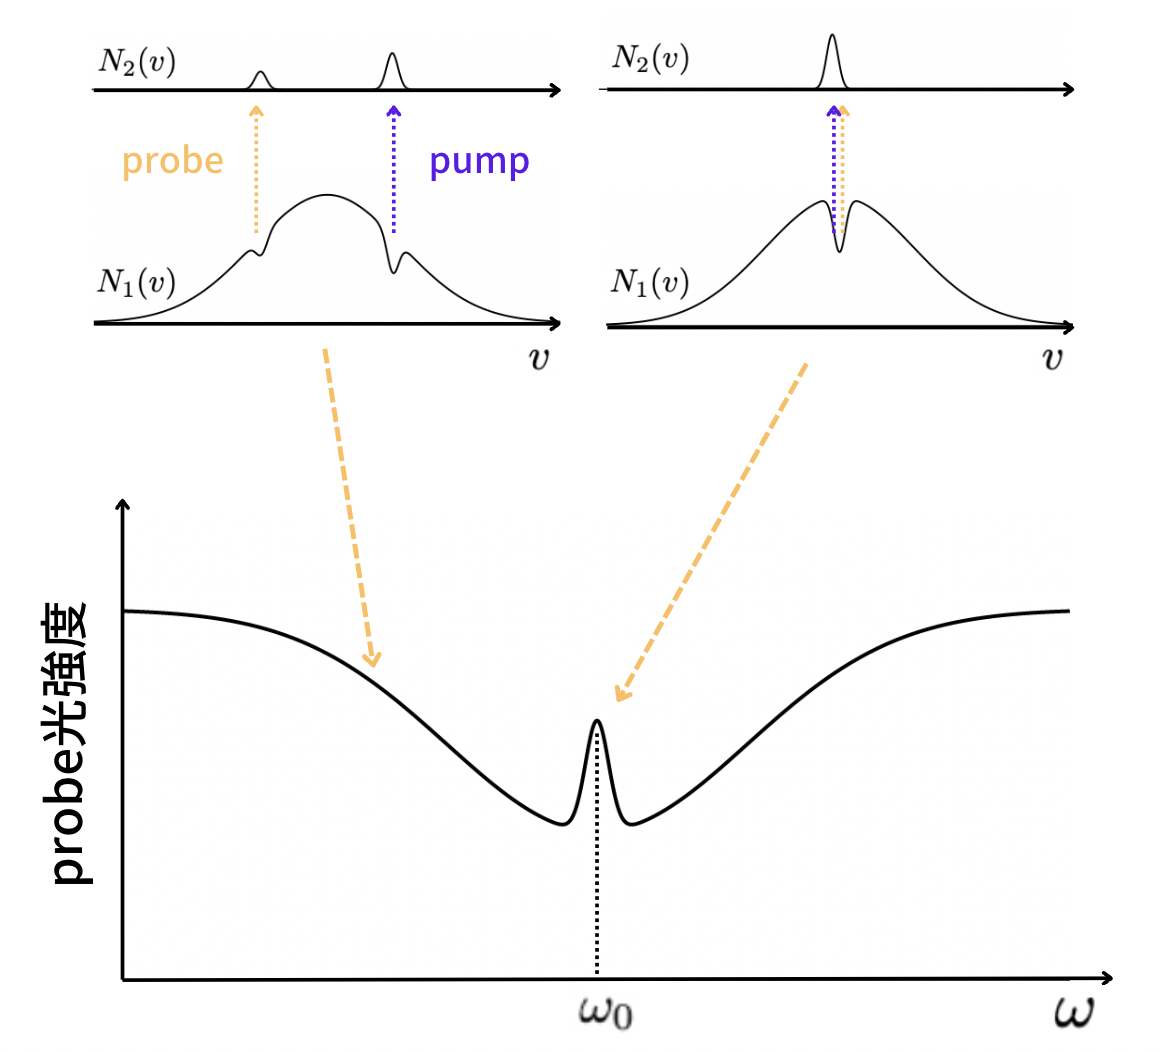
\includegraphics[width=0.6\textwidth]{images/sas_graph.png}
\caption{\label{fig:sas-graph}pump光とprobe光を吸収する原子が重なり、ラムディップができる}
\end{figure}
飽和吸収分光の概要を図\ref{fig:sas}に示す。偏光ビームスプリッタ(以下、PBS)によってレーザー光を強い光(pump)と弱い光(probe)に分け、原子のガスセル内で重ね合わせるようにしてprobe光を観測する。pump光の強度$I$は、飽和強度$I_{sat}$程度であるとする。

飽和吸収分光の原理について、簡単のため2準位系($N_1, N_2$)で説明する。pump光は速度$v = (\omega - \omega_0)/k$の原子と作用し、原子を$N_2$状態へ励起する。これにより、$N_1$状態の原子の速度分布には次のような幅を持つ穴ができる。\cite{foot}

\begin{equation}
\Delta\omega_{hole} = \Gamma \left( 1 + \frac{I}{I_{sat}} \right) ^ \frac{1}{2}
\end{equation}

ここで、$\Gamma$は励起状態の寿命に依存する自然広がりである。レーザー周波数が共鳴周波数から充分($(\omega - \omega_0) \ll \Delta\omega_{hole}$)離れている時、pump光とprobe光は速度が異なる原子と相互作用するため互いに影響しない。しかしレーザー周波数が共鳴周波数付近($\omega \simeq \omega_0$)の時、二つのレーザー光はどちらも$v \simeq 0$の原子と相互作用する。すなわち、pump光の吸収によってprobe光を吸収できる$N_1$状態の原子数が減少するため、probe光の透過高強度が大きくなるのである。これを観測すると図\ref{fig:sas}右下のようにドップラー広がりの頂点に鋭い窪みができる。このくぼみは、ラムディップと呼ばれ、自然広がり程度のドップラーフリーな信号である。

\subsection{クロスオーバー共振}
\begin{figure}
\centering
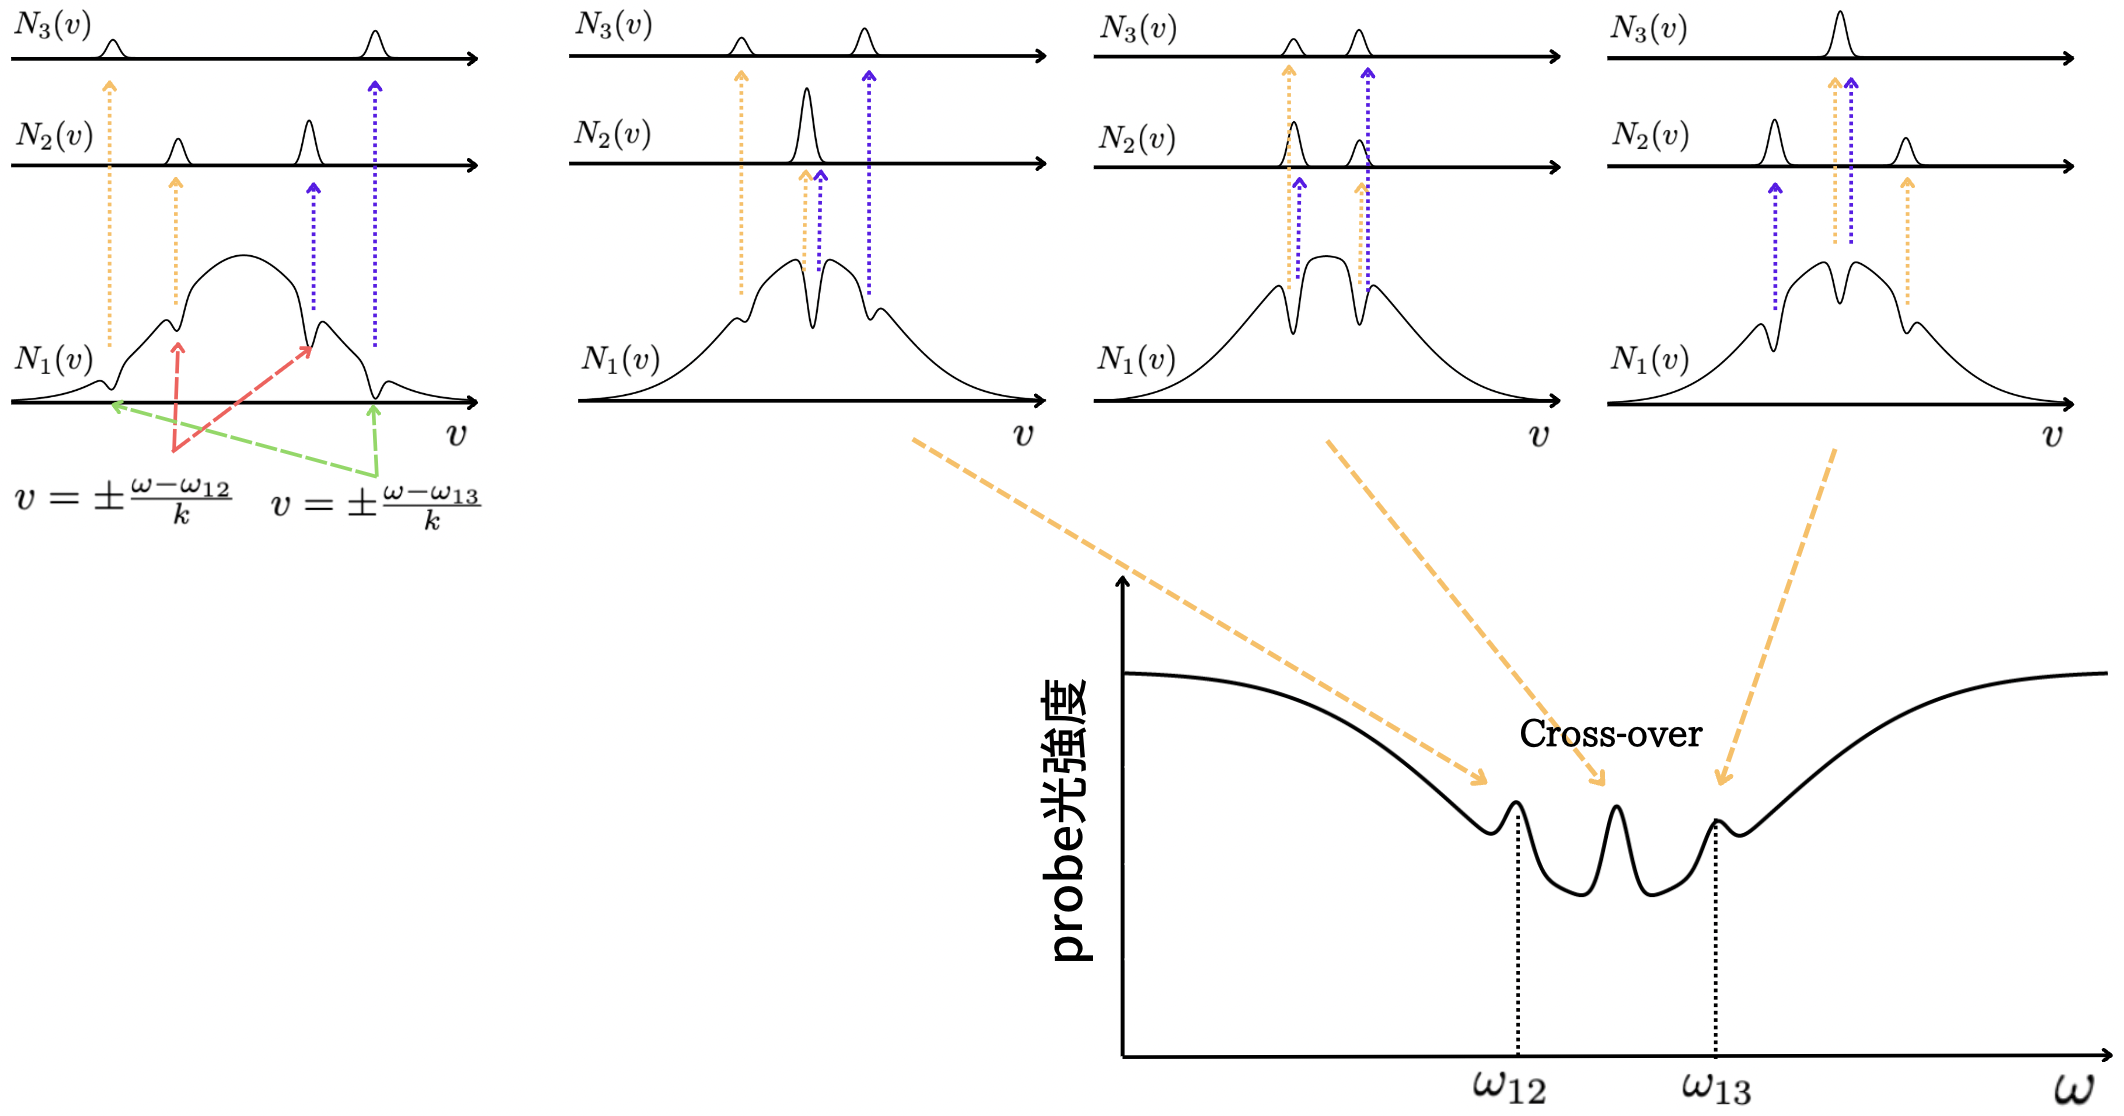
\includegraphics[width=1\textwidth]{images/cross-over_graph.png}
\caption{\label{fig:cross-over}クロスオーバー共振}
\end{figure}
実際の飽和吸収分光では、超微細構造によるエネルギー準位の分裂によって、ドップラー吸収の範囲内で複数の共鳴周波数が存在する。この時、二つの共鳴周波数の間にクロスオーバーディップと呼ばれる新たなピークが現れる現象について説明する。原子が$E_1, E_2, E_3(E_1 < E_2 < E_3)$の3つのエネルギー準位を持ち、各状態の原子数$N_1(v), N_2(v), N_3(v)$と表す。この時、$N_1\leftrightarrow N_2$の遷移は$v = (\omega - \omega_{12})/k$の速度成分を持つ原子で、$N_1\leftrightarrow N_3$の遷移は$v = (\omega - \omega_{13})/k$の速度成分を持つ原子で生じる。前節の飽和吸収分光の原理によると、レーザー周波数$\omega = \omega_{12}, \omega_{13}$の時にラムディップが現れる。しかし、図\ref{fig:cross-over}にあるように、$\omega = \left(\omega_{12} + \omega_{13} \right) / 2$の時、pump光の$N_1\leftrightarrow N_2$遷移はprobe光の$N_1\leftrightarrow N_3$遷移を減少させ、pump光の$N_1\leftrightarrow N_3$遷移はprobe光の$N_1\leftrightarrow N_2$遷移を減少させる。したがって、$\omega = \left(\omega_{12} + \omega_{13} \right) / 2$でピークが観測されるのである。

\subsection{変調移行分光(Modulation Transfer Spectroscopy)}
レーザーの周波数をロックするためには、飽和吸収信号を共鳴周波数の前後で正負が異なるようなエラー信号に変換してECDLにフィードバックする必要がある。エラー信号を得る技術はいくつか存在するが、その中でも変調移行分光法は急な信号勾配と高い周波数識別性を持つため、レーザーを狭い周波数にロックすることができる。なお、本節の議論は\cite{mt}\cite{mt2}を参考にしている。

\begin{figure}
\centering
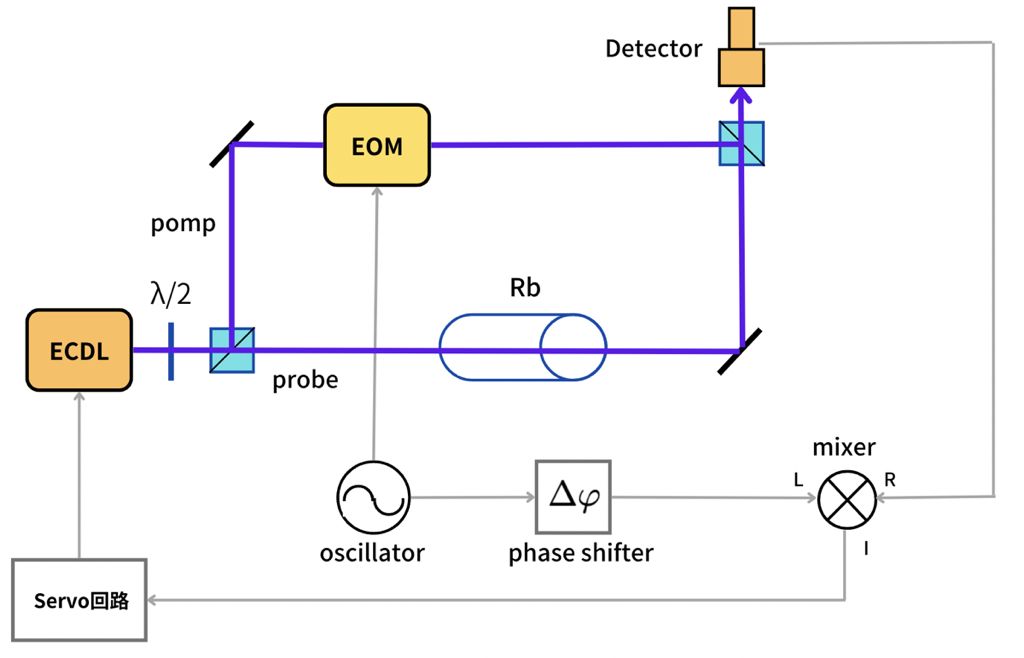
\includegraphics[width=0.9\textwidth]{images/mt.png}
\caption{\label{fig:mt}変調移行分光}
\end{figure}

変調移行分光の概要を図\ref{fig:mt}に示す。飽和吸収分光の光学系に加えて、pump光の光路にEOM(電気光学変調機)が設置されている。PDで得られた信号と変調に用いたRF信号をmixerで掛け合わせることでエラー信号が得られ、Servo回路を通してECDLにフィードバックしている。phase shifterはmixerに入れるRF信号の位相をきれいなエラー信号が得られるように調整する役割を果たしている。以下、エラー信号が得られる原理について述べる。

EOMに周波数$\omega_m$のRF信号を入れると、周波数$\omega$のpump光の光電場は変調され、以下のように表せる。

\begin{align}
\begin{split}
    E &= 
        E_0 \exp i \left[{\omega t + \delta \sin{(\omega_m t)}} \right] \\
    &= E_0e^{i\omega t} \sum_{n = -\infty}^\infty J_n(\delta) e^{in\omega_m t} \\
    &= E_0 \left[ J_0(\delta)e^{i\omega t} + J_1(\delta)e^{i(\omega + \omega_m)t} - J_1(\delta)e^{i(\omega - \omega_m)t} + \cdots \right]
\end{split}
\end{align}

ここで$\delta$は変調指数、$J_n$は$n$次のBessel関数である。一般に$\delta < 1$であり、probe光は周波数$\omega$の光に、周波数$\omega \pm \omega_{m}$の一次のサイドバンドが加わった光となる。変調されたpump光は、変調されていないprobe光と蒸発Rbセル内で対向して入射し重ね合わされる。ここで、レーザー光が原子の共鳴周波数付近の時、原子気体の非線形光学現象である四光波混合という現象によって、pump光の各サイドバンドに対してprobe光に変調が移行する。四光波混合の詳細な原理については\cite{four-wave}などを参照されたい。変調移行はサブドップラー共鳴条件が満たされる時のみ起こるため、エラー信号のベースラインはドップラー吸収効果に依存しない平坦な信号となる。偏光、温度、ビーム強度の変動による吸収の変化に影響されないのが変調移行分光法の大きな利点である。元のprobe光とprobe光のサイドバンドは干渉し、Photo Diode上で次のビート信号が検出される。

\begin{align}
\begin{split}
    S(\omega_m) &= 
        \frac{C}{\sqrt{\Gamma^2 + \omega_m^2}} \sum_{n = -\infty}^\infty J_n(\delta)J_{n-1}(\delta) \\
    &\times \lbrack L_{(n+1)/2} + L_{(n-2)/2} \cos{\left( \omega_m t + \phi \right)} \\
    &+ D_{(n+1)/2} + D_{(n-2)/2} \sin{\left( \omega_m t + \phi \right)} \rbrack + Const + \mathcal{O}(e^{2i\omega_m t})
\end{split}
\end{align}

ここで、

\begin{align}
\begin{split}
&L_n = \frac{\Gamma^2}{\Gamma^2 + \left( \Delta - n\omega_m \right)^2}, \\
&D_n = \frac{\Gamma(\Delta - n\omega_m)}{\Gamma^2 + \left( \Delta - n\omega_m \right)^2}
\end{split}
\end{align}

であり、$\Gamma$は自然線幅、$\Delta$は共鳴周波数からの離調、$\phi$はpump光にかけたRF信号に対する位相である。今、$\delta < 1$であり2次以降のサイドバンドは無視できると仮定すると、式(\ref{MT_signal})は次のように具体化される。

\begin{align}
\begin{split}
\label{MT_signal}
    S(\omega_m) &= 
        \frac{C}{\sqrt{\Gamma^2 + \omega_m^2}} J_0(\delta)J_1(\delta) \\
    &\times \lbrack (L_{-1} + L_{-1/2} + L_{1/2} - L_1) \cos{\left( \omega_m t + \phi \right)} \\
    &+ (D_{1} + D_{-1/2} - D_{1/2} + D_{-1}) \sin{\left( \omega_m t + \phi \right)} \rbrack + Const + \mathcal{O}(e^{2i\omega_m t})
\end{split}
\end{align}

この信号を位相シフトしたRF信号と共にmixerで掛け合わせることで、sin項またはcos項に含まれるエラー信号を復調することができる。定数項と$\mathcal{O}(e^{2i\omega_m t})$はServo回路がローパスフィルターの働きもするため切り捨てられる。結果として、sin項、cos項共にエラー信号は離調$\Delta$に依存した奇関数となる。$\omega_m \leq \Gamma$の時、信号は共鳴周波数でゼロクロスする急な勾配を持った関数となり、レーザーのロックに理想的な信号となる。

\clearpage
\section{電磁場誘起透明化(Electromagnetically Induced Transparency)}
電磁場誘起透明化(Electromagnetically induced transparency, 以下EIT)とは、3つ以上のエネルギー準位を持つ系に対してその吸収波長を持つ光を入射することで生じる量子干渉効果により、系の固有状態が見かけ上光の吸収や放出に関与しなくなる、すなわち物質が透明化する現象である。ここでは3準位原子のモデルと2本の光との相互作用を考え、原子がその光に対して透明化するまでの仕組みを説明する。なお、本節は参考文献\cite{eit-pertubation}\cite{eit-absorption}の説明を参考にしている。
\subsection{運動方程式の記述}
\begin{figure}[hbtp]
\centering
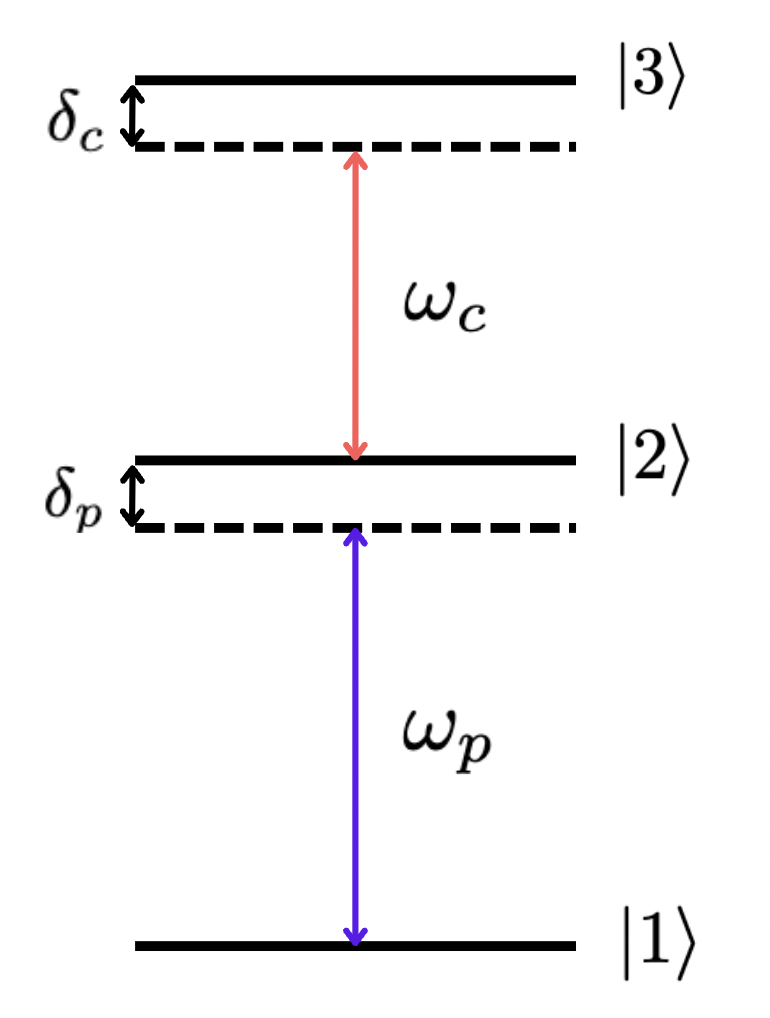
\includegraphics[width=0.4\textwidth]{images/EIT_spectre.png}
\caption{\label{fig:eit-spectre}3準位系のエネルギー図}
\end{figure}

図\ref{fig:eit-spectre}のような3準位系を持つ原子に対して、$| 1 \rangle$, $| 2 \rangle$間に共鳴するprobe光と、$| 2 \rangle$, $| 3 \rangle$間に共鳴するcoupling光を入射する場合を考える。この系に対するハミルトニアンは非摂動ハミルトニアン$H_0$とレーザー光と原子の相互作用ハミルトニアン$H_{int}$の和で与えられる。

\begin{align}
\begin{split}
H &= H_0 + H_{int} \\
&= 
    \begin{pmatrix} 
        W_3 & 0 & 0 \\
        0 & W_2 & 0 \\
        0 & 0 & W_1 \\
    \end{pmatrix}
    +
    \begin{pmatrix} 
        0 & \mathcal{H}_{32} & 0 \\
        \mathcal{H}_{23} & 0 & \mathcal{H}_{21} \\
        0 & \mathcal{H}_{12} & 0 \\
    \end{pmatrix}
\end{split}
\end{align}
ここで、$W$は各準位の固有エネルギーであり、
\begin{equation}
    \omega_{ij} = (W_i - W_j) / \hbar
\end{equation}
である。また、
\begin{equation}
\begin{split}
\mathcal{H}_{12} &= -p_{12}E_p\\
&= -p_{12} \varepsilon_p \cos{(\omega_p t)} \\
&= -\hbar \Omega_p \cos{(\omega_p t)} \\
\mathcal{H}_{23} &= -p_{23}E_c \\
&= -p_{23} \varepsilon_c \cos{(\omega_c t)} \\
&= -\hbar \Omega_c \cos{(\omega_c t)} \\
&\left( \Omega_p \equiv \frac{p_{12}\varepsilon_p}{\hbar} , \Omega_c \equiv \frac{p_{23}\varepsilon_c}{\hbar} \right) 
\end{split}
\end{equation}
である。ここで、$E_p, E_c$はprobe光とcoupling光の電場、$\varepsilon_p, \varepsilon_c$は電場の振幅、$p_{ij}$は双極子モーメントを表しており、$\Omega_p, \Omega_c$は各状態間の遷移のラビ周波数である。ここからは密度行列$\rho$の時間変化を求める。
\begin{equation}
\rho = 
\begin{pmatrix} 
        \rho_{33} & \rho_{32} & \rho_{31} \\
        \rho_{23} & \rho_{22} & \rho_{21} \\
        \rho_{13} & \rho_{12} & \rho_{11} \\
\end{pmatrix}
\end{equation}
とおくと、密度演算子の運動方程式であるLiouville方程式は、
\begin{equation}
\dot{\rho} = \frac{1}{i\hbar} \lbrack \mathcal{H}, \rho \rbrack
\end{equation}
と書ける。$ij$成分については以下のように書ける。
\begin{equation}
\dot{\rho}_{ij} = \frac{1}{i\hbar} \sum_{n=1}^3 \lbrack \mathcal{H}_{in} \rho_{nj} - \rho_{in}\mathcal{H}_{nj} \rbrack
\end{equation}
ここまでの式から密度行列の運動方程式を計算する。
\begin{align}
{\dot{\rho}_{33}} &= i\left( \Omega_c^* {\rho_{23}} - {\rho_{32}}\Omega_c \right) \cos{(\omega_c t)} \\
{\dot{\rho}_{22}} &= i\left( \Omega_c^* {\rho_{32}} - {\rho_{23}}\Omega_c \right) \cos{(\omega_c t)} + i\left( \Omega_p^* {\rho_{12}} - {\rho_{21}}\Omega_p \right) \cos{(\omega_p t)} \\
{\dot{\rho}_{11}} &= i\left( \Omega_p {\rho_{21}} - {\rho_{12}}\Omega_p^* \right) \cos{(\omega_p t)} \\
{\dot{\rho}_{12}} &= i\lbrack {\rho_{12}}\omega_{21} + \Omega_p \cos{\omega_p t} ({\rho_{22}} - {\rho_{11}}) - {\rho_{13}} \Omega_c^* \cos{\omega_c t} \rbrack \\
{\dot{\rho}_{23}} &= i\lbrack {\rho_{23}}\omega_{32} + \Omega_c \cos{\omega_c t} ({\rho_{33}} - {\rho_{22}}) + {\rho_{13}} \Omega_p^* \cos{\omega_p t} \rbrack \\
{\dot{\rho}_{13}} &= i\lbrack {\rho_{13}}\omega_{31} + {\rho_{23}}\Omega_p \cos{\omega_p t} - {\rho_{12}}\Omega_c \cos{\omega_c t}  \rbrack
\end{align}
ここで、${\rho_{ij}}$を${\rho_{ij}^{'}}$と書き換え、密度行列が回転座標系に乗るとして以下のように変数変換する。
\begin{equation}
\begin{split}
{\rho_{12}^{'}} &= \rho_{12}e^{i\omega_p t} \\
{\rho_{23}^{'}} &= \rho_{23}e^{i\omega_c t} \\
{\rho_{13}^{'}} &= \rho_{13}e^{i(\omega_p + \omega_c) t} 
\end{split}
\end{equation}
さらにオイラーの公式を用いれば、例えば${\dot{\rho}_{33}}$は以下のようになる。
\begin{equation}
\begin{split}
    \dot{\rho}_{33} &= i\left( \Omega_c^* {\rho_{23} e^{i\omega_c t}} - {\rho_{32}}\Omega_c e^{-i\omega_c t} \right) \frac{e^{i\omega_c t} + e^{-i\omega_c t}}{2} \\
    &= \frac{i}{2} \lbrack \Omega_c^* {\rho_{23}} -  {\rho_{32}}\Omega_c + \Omega_c^* {\rho_{23}e^{2i\omega_c t}} - {\rho_{32}}\Omega_c e^{-2i\omega_c t} \rbrack
\end{split}
\end{equation}
この時、回転波近似によって$e^{\pm 2i\omega_c t}$の項は無視できる。ここで、現象論に従って以下のような緩和項をLiouville方程式に付け加える。
\begin{equation}
    \dot{\rho} = \frac{1}{i\hbar} \lbrack \mathcal{H}, \rho \rbrack + \dot{\rho}_{\text{relax}}
\end{equation}
\begin{equation}
    \dot{\rho}_{\text{relax}} = 
    \begin{pmatrix} 
        -\Gamma_3 \rho_{33} & -\gamma_{32}\rho_{32}  & -\gamma_{31}\rho_{31}  \\
        -\gamma_{23}\rho_{23} & -\Gamma_2 \rho_{22}  &  -\gamma_{21} \rho_{21}  \\
        -\gamma_{13}\rho_{13} & -\gamma_{12} \rho_{12} & \Gamma_2 \rho_{22} \\
    \end{pmatrix}
\end{equation}
ここで、$\Gamma_2$と$\Gamma_3$はそれぞれ状態$| 2 \rangle$と$| 3 \rangle$からの自然放出による緩和、$\gamma$はコヒーレンスの緩和であり、$\gamma_{ij} = (\Gamma_i + \Gamma_j) / 2$である。$| 1 \rangle$, $| 3 \rangle$間はパリティが同じため直接緩和が起きず、$\Gamma_1 = 0$である。あらためて密度行列の運動方程式を計算すると、
\begin{align}
\label{dot-rho-33}
{\dot{\rho}_{33}} &= \frac{i}{2} \left( \Omega_c^* {\rho_{23}} - \Omega_c{\rho_{32}} \right) - \Gamma_3 \rho_{33} \\
{\dot{\rho}_{22}} &= -\frac{i}{2} \lbrack \Omega_c^* {\rho_{23}} - \Omega_c{\rho_{32}} \rbrack + \frac{i}{2} \lbrack \Omega_p^* {\rho_{12}} - \Omega_p{\rho_{21}} \rbrack - \Gamma_2 \rho_{22} \\
{\dot{\rho}_{11}} &= \frac{i}{2} \left( \Omega_p {\rho_{21}} - \Omega_p^*{\rho_{12}} \right) + \Gamma_2 \rho_{22} \\
{\dot{\rho}_{12}} &= \frac{i}{2} \lbrack \Omega_p (\rho_{22} - \rho_{11}) - \Omega_c^* \rho_{13} \rbrack + \left( i\delta_p -\gamma_{12} \right) \rho_{12} \\
{\dot{\rho}_{23}} &= \frac{i}{2} \lbrack \Omega_c (\rho_{33} - \rho_{22}) + \Omega_p^* \rho_{13} \rbrack + \left( i\delta_c -\gamma_{23} \right) \rho_{23} \\
\label{dot-rho-11}
{\dot{\rho}_{13}} &= \frac{i}{2} \lbrack \Omega_p \rho_{23} - \Omega_c \rho_{12} \rbrack + \left( i\delta_0 -\gamma_{13} \right) \rho_{13}
\end{align}
となる。ここで、
\begin{equation}
\begin{split}
    \delta_p &\equiv \omega_{21} - \omega_p \\
    \delta_c &\equiv \omega_{32} - \omega_c \\
    \delta_0 &\equiv \omega_{31} - (\omega_p + \omega_c) \\
    &= \delta_p + \delta_c
\end{split}
\end{equation}
とおいた。この方程式の解は、摂動論によって近似的に解かれる。

\subsection{摂動理論を用いた解釈}
ここからはprobe光が遥かに弱い($\Omega_p \ll \Omega_c$)ことを仮定し、摂動理論を適用して解を求めていく。定常状態の解は式(\ref{dot-rho-33})〜(\ref{dot-rho-11})において、時間微分を0とおくことで求められる。さらに
\begin{equation}
\begin{split}
    {\gamma_{12}^{'}} &\equiv \gamma_{12} - i\delta_p \\
    {\gamma_{23}^{'}} &\equiv \gamma_{23} - i\delta_c \\
    {\gamma_{13}^{'}} &\equiv \gamma_{13} - i\delta_0
\end{split}
\end{equation}
とおくと、
\begin{align}
\rho_{33} &= \frac{1}{\Gamma_3} \frac{i}{2} \left( \Omega_c^* {\rho_{23}} - \Omega_c{\rho_{32}} \right) \\
\label{rho-22}
\rho_{22} &= \frac{1}{\Gamma_2} \frac{i}{2} \left( \Omega_p^* {\rho_{12}} - \Omega_p{\rho_{21}} \right) \\
\label{rho-12}
\rho_{12} &= \frac{1}{\gamma_{12}^{'}} \frac{i}{2} \lbrack \Omega_p (\rho_{22} - \rho_{11}) - \Omega_c^* \rho_{13} \rbrack \\
\label{rho-23}
\rho_{23} &= \frac{1}{\gamma_{23}^{'}} \frac{i}{2} \lbrack \Omega_c (\rho_{33} - \rho_{22}) + \Omega_p^* \rho_{13} \rbrack \\
\rho_{13} &= \frac{1}{\gamma_{13}^{'}} \frac{i}{2} \lbrack \Omega_p \rho_{23} - \Omega_c \rho_{12} \rbrack
\end{align}
となる。0次の解はprobe光、coupling光を入射していない場合なので、状態$| 1 \rangle$の分布数が1、すなわち$\rho_{11}^{(0)} = 1$, $\rho_{22}^{(0)} = \rho_{33}^{(0)} = 0$である。これを代入することによって1次の解を求める。ここでは$\rho_{12}^{(1)}$のみが解を持つ。式(\ref{rho-12})より、
\begin{equation}
\label{rho-12-1}
    \rho_{12}^{(1)} = - \frac{i}{2} \frac{\Omega_p}{\gamma_{12}^{'}}
\end{equation}
が得られる。この解は$\Omega_p$に比例しているので線形吸収を表している。

式(\ref{rho-12-1})を代入することにより、2次の解である$\rho_{22}^{(2)}$, $\rho_{11}^{(2)}$, $\rho_{13}^{(2)}$が求められる。式(\ref{rho-22})より、
\begin{equation}
\begin{split}
\label{rho-22-2}
    \rho_{22}^{(2)} &= \frac{1}{4}\frac{|\Omega_p|^2}{\Gamma_2} \left( \frac{1}{\gamma_{12}^{'}} + \frac{1}{{\gamma_{12}^{'}}^*} \right) \\
    &= \frac{1}{4}\frac{|\Omega_p|^2}{\Gamma_2} \frac{2\gamma_{12}}{\gamma_{12}^2 + \delta_{p}^2} \\
    &= \frac{1}{2}\frac{|\Omega_p|^2}{\Gamma_2 \gamma_{12}} \mathcal{L}_p
\end{split}
\end{equation}
ただし、
\begin{equation}
    \mathcal{L}_p \equiv \frac{\gamma_{12}^2}{\gamma_{12}^2 + \delta_{p}^2}
\end{equation}
とおいた。$\rho_{11}^{(2)}$については、$\rho_{11}^{(2)} = -\rho_{22}^{(2)}$となるので、
\begin{equation}
\label{rho-11-2}
\rho_{11}^{(2)} = -\frac{1}{2} \frac{|\Omega_p|^2}{\Gamma_2 \gamma_{12}} \mathcal{L}_p
\end{equation}
となる。式(\ref{rho-23})より
\begin{equation}
\label{rho-13-2}
\rho_{13}^{(2)} = -\frac{1}{4}\frac{\Omega_p \Omega_c}{\gamma_{12}^{'} \gamma_{13}^{'}} 
\end{equation}
式(\ref{rho-22-2}), (\ref{rho-11-2}), (\ref{rho-13-2})を代入することにより、3次の解である$\rho_{12}^{(3)}$, $\rho_{23}^{(3)}$が求められる。
\begin{align}
\label{rho-12-3}
\rho_{12}^{(3)} &= \frac{i}{2} \frac{|\Omega_p|^2 \Omega_p}{\Gamma_2 \gamma_{12} \gamma_{12}^{'}} \mathcal{L}_p +  \frac{i}{8} \frac{|\Omega_c|^2 \Omega_p}{\gamma_{12}^{'2} \gamma_{13}^{'}} \\
\rho_{23}^{(3)} &= -\frac{i}{4} \frac{|\Omega_p|^2 \Omega_c}{\Gamma_2 \gamma_{12} \gamma_{23}^{'}} \mathcal{L}_p -  \frac{i}{8} \frac{|\Omega_p|^2 \Omega_c}{\gamma_{12}^{'} \gamma_{23}^{'} \gamma_{13}^{'}}
\end{align}
同様にして4次の解、5次の解を求め、$\rho_{12}$の摂動項の和をとることで、$\rho_{12}$は以下のように求められる。\cite{eit-absorption}
\begin{equation}
    \rho_{12} = \frac{i\Omega_p}{8\gamma_{12}^{'}\gamma_{13}^{'} + 2|\Omega_c|^2}
\end{equation}


\subsection{吸収係数}
電磁気学によれば、電気感受率の虚部は誘電体による電場のエネルギーの吸収を表す。\cite{nagaoka-yosuke}したがって、probe光の吸収に関する電気感受率を求めることで、probe光の吸収を表すことができる。

電場$E$によって作られる分極$P$は以下のように表される。
\begin{equation}
    P = \epsilon_0 \chi E
\end{equation}
ここで$\epsilon_0$は真空の誘電率、$\chi$は電気感受率である。また,単位体積当たり$N$個の原子の巨視的な双極子モーメントの期待値は以下のように表される。
\begin{equation}
\begin{split}
    P &= N\langle p \rangle \\
    &= N(\rho_{12}p_{21} + \rho_{23}p_{32} + c.c.)
\end{split}
\end{equation}
probe光の周波数$\omega_p$で振動する成分を考えると、
\begin{equation}
     \epsilon_0 \chi \varepsilon_p = N\rho_{12}p_{21} 
\end{equation}
という関係が成り立つ。したがって、
\begin{equation}
\begin{split}
    \chi &=  \frac{N\rho_{12}p_{21}}{\epsilon_0 \varepsilon_p} \\
    &= \frac{N |p_{12}|^2}{\epsilon_0 \hbar \Omega_p}\rho_{12}
\end{split}
\end{equation}
となる。適当な係数を与えることで電場の吸収は$\text{Im}\lbrack \Gamma_2 \rho_{12} /\Omega_p \rbrack$に比例し、吸収係数$\alpha$は、
\begin{equation}
\begin{split}
\label{eit-absorption}
    \alpha &=  \text{Im} \lbrack \frac{\Gamma_2 \rho_{12}}{\Omega_p} \rbrack \\
    &= \text{Im} \lbrack \frac{\Gamma_2}{\Omega_p} \frac{i\Omega_p}{8\gamma_{12}^{'}\gamma_{13}^{'} + 2|\Omega_c|^2} \rbrack \\
    &= \frac{\Gamma_2 \left( \Gamma_2\Gamma3 - 4\delta_p\delta_0 \right)}{8\left[ (\Gamma_2^2 + 4\delta_p^2)(\Gamma_3^2 + 4\delta_0^2) + 2|\Omega_c|^2 \right]} \\
\end{split}
\end{equation}
となる。coupling光の離調がゼロ、すなわち$\delta_0 = \delta_p$とすると、probe光の離調と吸収の関係は図\ref{fig:absorption}のようになる。
\begin{figure}[hbtp]
\centering
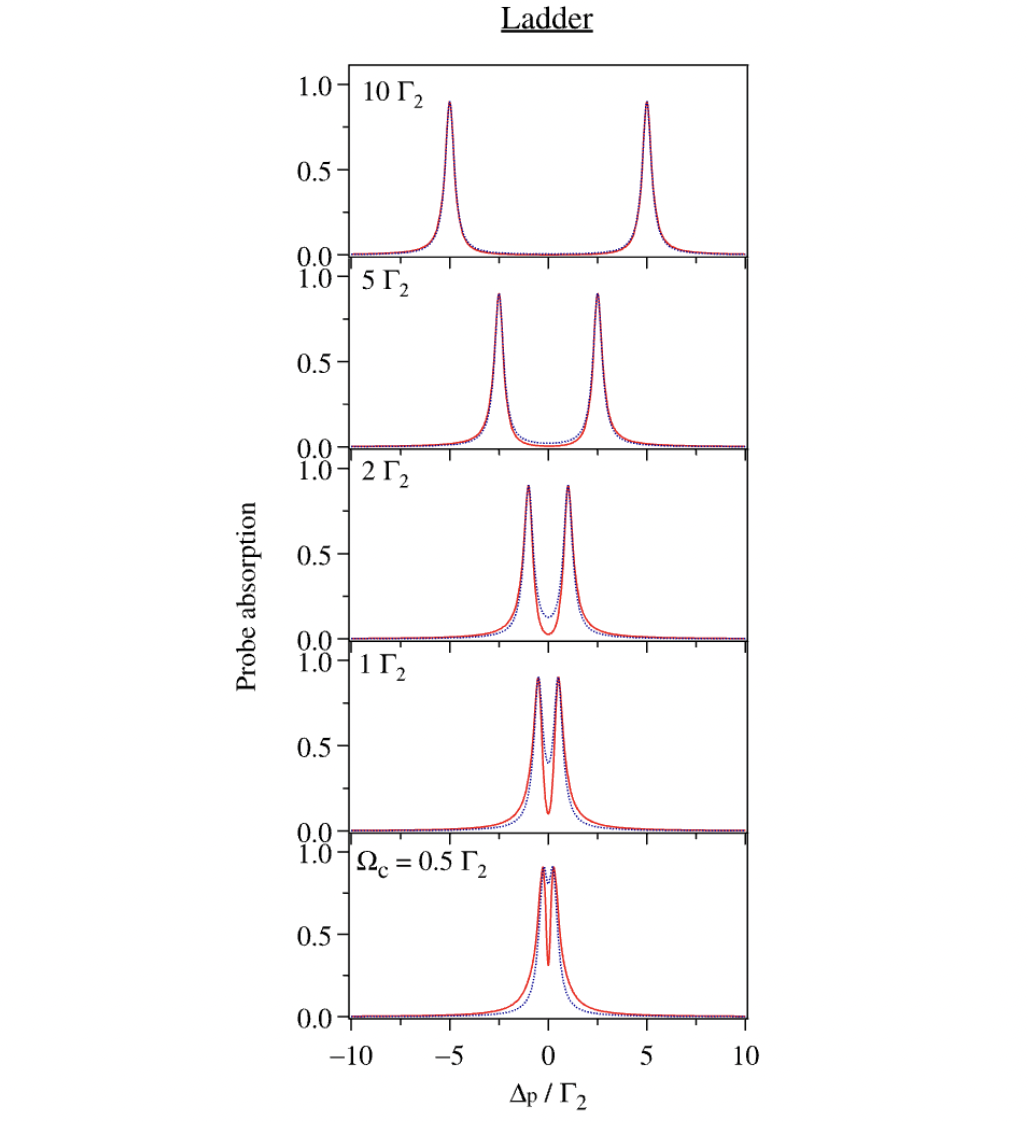
\includegraphics[width=0.8\textwidth]{images/eit_absorption.png}
\caption{\label{fig:absorption} ラダー型EIT信号 $\delta_c = 0$の時のprobe光のスペクトルを、$\Omega_c$の値によって5通り示している。実線は密度行列の完全解を表しており、点線はドレスト状態による影響を受けた実際に観測されるスペクトルを表す \cite{eit-absorption}より引用。}
\end{figure}

EITは、強いcoupling光によって原子のエネルギー準位がシフトし、新たな固有状態(ドレスト状態)が生まれることによって起こる。しかし、ドレスト状態の内のダークステートと呼ばれる光の吸収・放出が起こらない固有状態は、ドレスト状態の(への)自然崩壊との相互作用によって安定ではない。この影響によって、特に$\Omega_c$が$\Gamma_2$に比べて小さくなるほど、観測されるEITピークは小さくなる。

\clearpage
\chapter{実験系の構築}
この章では、初めに我々が構築した実験系の概要についてまとめる。その後、それらの構成要素である外部共振器型半導体レーザー、周波数安定化システムについて詳細を述べる。電磁誘起透明化(EIT)信号の観測に関しては、次の章で詳細を述べる。
\section{実験系の概要}
% TODO:Rbセルのサイズ
実験系の概要、及び光学系の写真を図\ref{fig:all},\ref{fig:all_real}に示す。ECDL1は$(\lambda \simeq 420)$nm、ECDL2は$(\lambda \simeq 1020)$nmである。各レーザーから出た光は、戻り光をカットするためアイソレーターに通されている。ECDL1の方のアイソレーターの実験スペックは、$\text{Transmission:} 80.4\%, \text{Isolation:} -34.4\text{dB}$であった。ECDL2の方のアイソレーターの実験スペックは、$\text{Transmission:} 35.8\%, \text{Isolation:} -15.4\text{dB}$であった。少し性能が悪い理由として、アイソレーターが回転できない固定型の製品だったため、入射する光の偏光に対してアイソレーターの角度を最適化できていないことが考えられる。また、ECDL1の方のアイソレーターには、カットされた光が外部に放出される穴が開いており、目などにレーザー光が入らないよう遮光シートを被せた。この遮光シートを被せないと各実験で観測するprobe光に明らかにノイズが増えるので、アイソレーター内での光の干渉を防ぐために重要な効果があると考える。

ECDL1から出た光は、アイソレーターを通った後、$\lambda/2$波長板とPBSによって周波数安定化のための変調移行分光の光学系へと光が分けられる。変調移行分光の光学系については、図\ref{fig:mt}に示した通りである。PBSを真っ直ぐ通過した光はさらに$\lambda/2$波長板とPBSによって分けられ、それぞれEIT信号観測実験の系と、波長系へと繋がる光ファイバーに向かっている。

ECDL2から出た光は、アイソレーターを通った後、波長板とPBSによってEIT信号観測実験の系へと光が分けられ、残りの光は波長系へと繋がる光ファイバーに通されている。

\begin{figure}[hbtp]
\centering
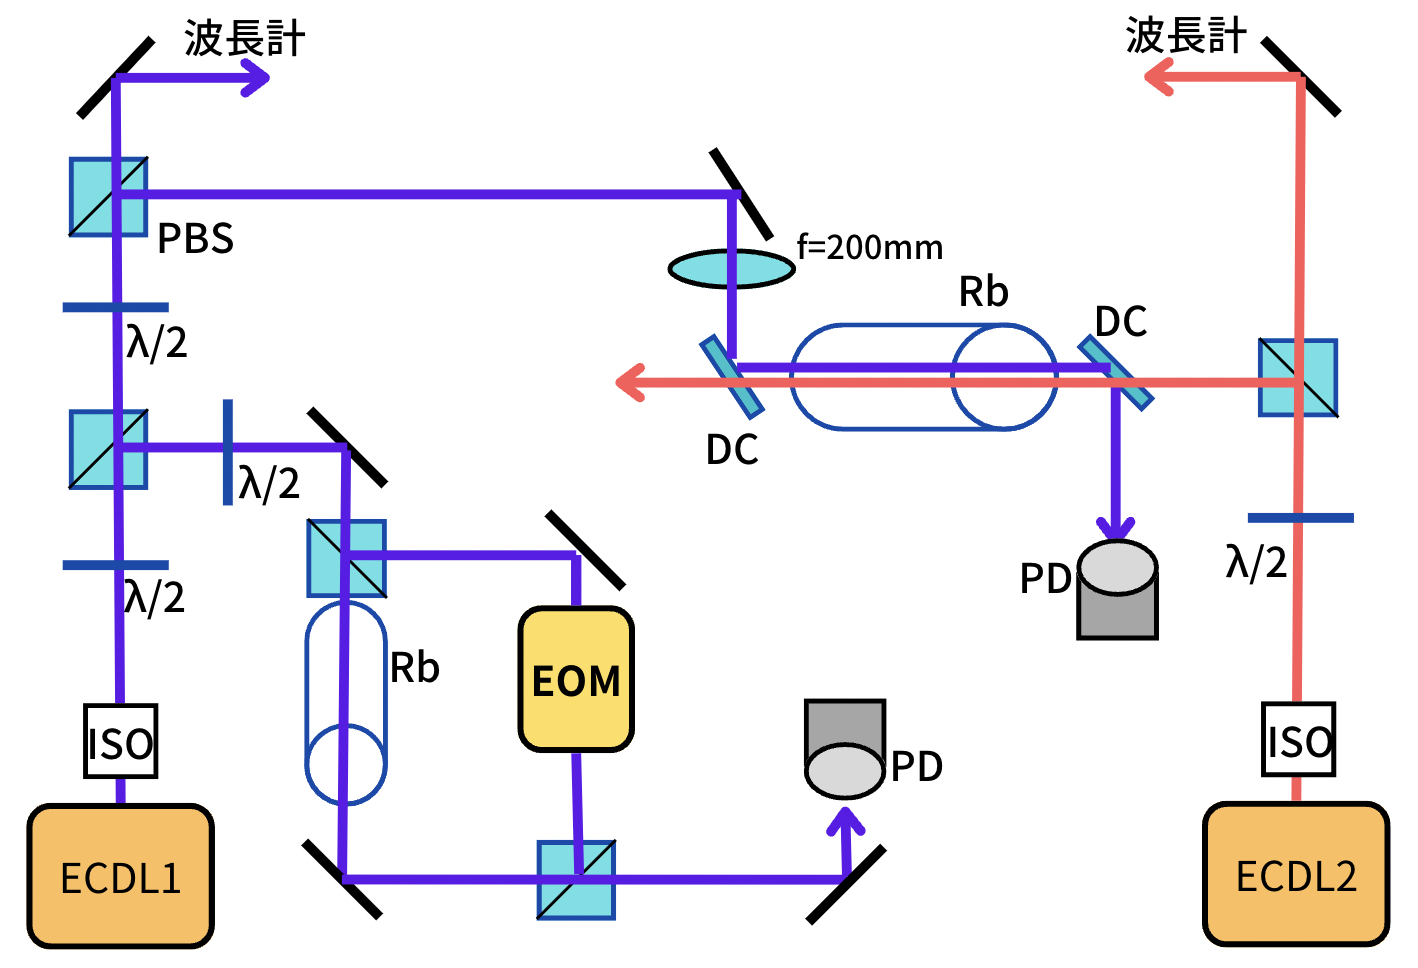
\includegraphics[width=0.8\textwidth]{images/all.png}
\caption{\label{fig:all}光学系の概要 ISO:アイソレーター、$\lambda / 2$:波長板、PBS:偏光ビームスプリッター、DC:ダイクロイックミラー、PD:フォトダイオード、EOM:電気光学変調機}
\end{figure}

\begin{figure}[hbtp]
\centering
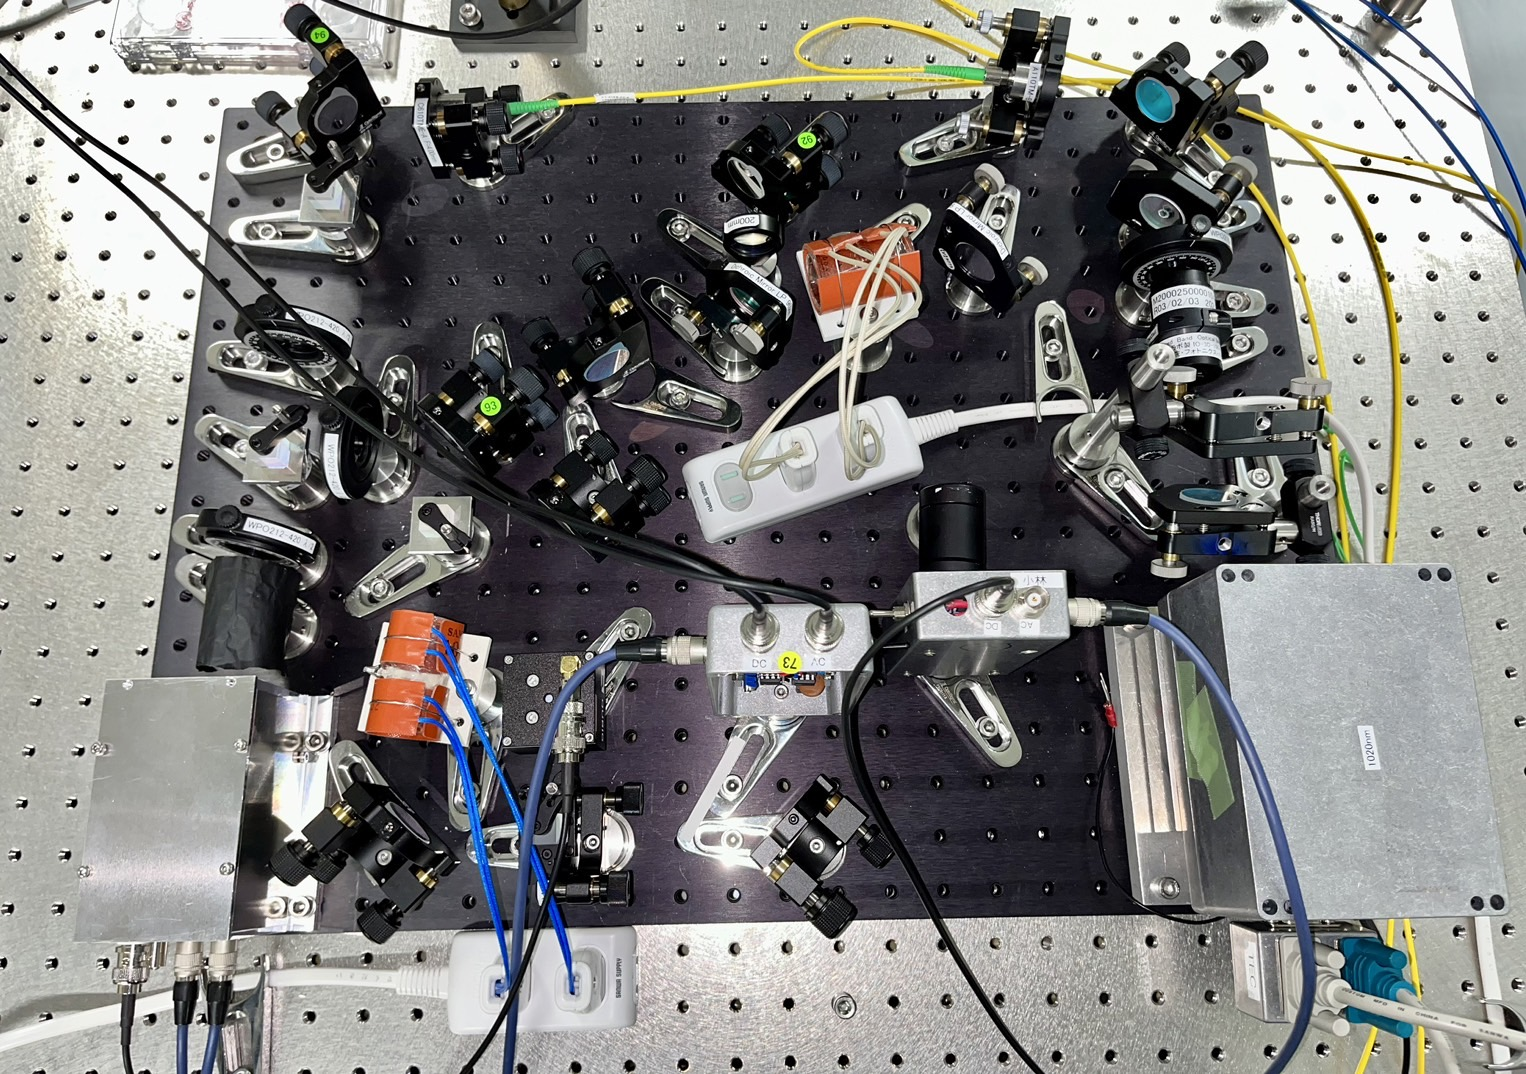
\includegraphics[width=0.8\textwidth]{images/all_real.jpg}
\caption{\label{fig:all_real}光学系の写真}
\end{figure}

\clearpage
\section{外部共振器型半導体レーザー(ECDL)}
レーザー(Laser)は、「放射の誘導放出による光の増幅(Light amplification by stimulated emission of radiation)」の頭文字を集めて作った造語であることからもわかるように、半導体結晶から放出された光を誘導放出により増幅させた光源である。反射鏡等で光の一部をフィードバックし共振器を形成することで、特定の波長の光が選択的に増幅され「発振」する。\cite{yamamotomasashi}

\begin{figure}[hbtp]
\centering
\begin{minipage}[b]{0.4\linewidth}
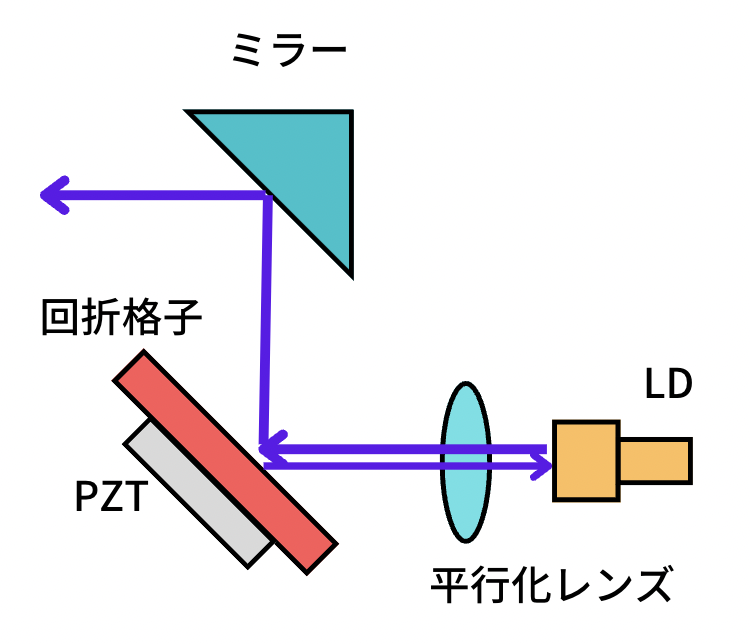
\includegraphics[width=1\textwidth]{images/ecdl.png}
\end{minipage}
\begin{minipage}[b]{0.45\linewidth}
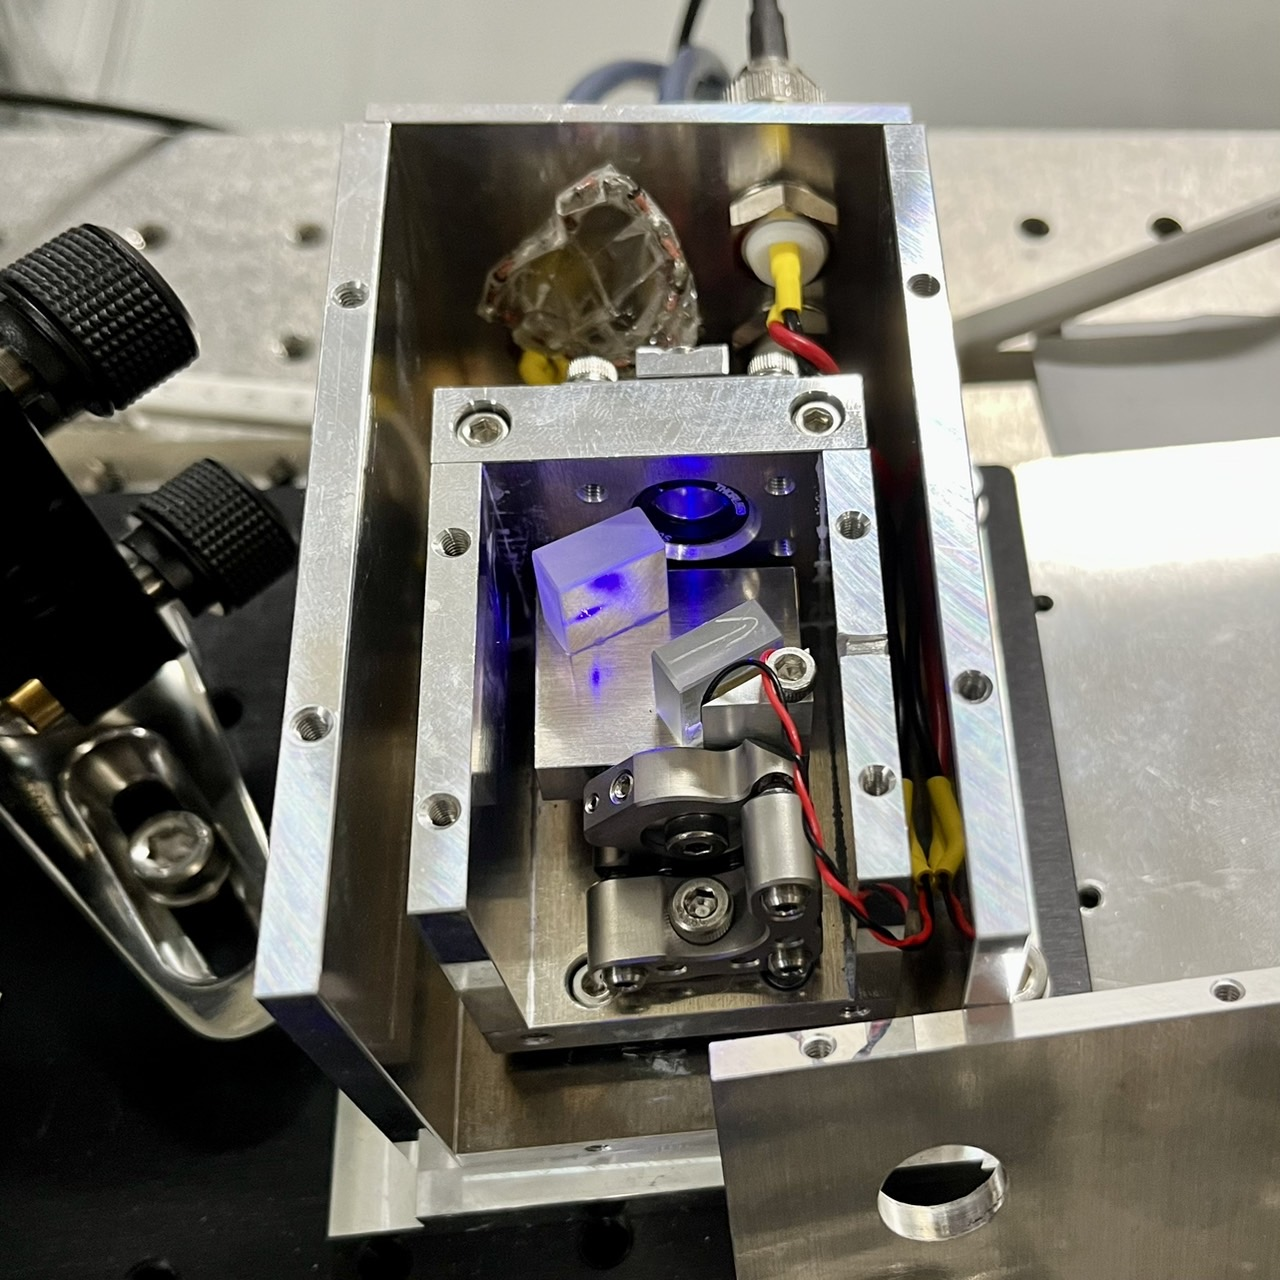
\includegraphics[width=1\textwidth]{images/ecdl_real.jpg}
\end{minipage}
\caption{\label{fig:ecdl}(左)ECDLの概要 (右)実際に作成した420nm ECDL}
\end{figure}

外部共振器型半導体レーザー (External Cavity Diode Laser: ECDL) とは実効的な共振器長を大きくすることで線幅を狭くしている半導体レーザー光源である。\cite{suzuki}本実験で作成したECDLの概要を図\ref{fig:ecdl}に示す。LD素子から出力された光は、コリメーションレンズ(f=4.51mm)を通して平行光になり、グレーティングと呼ばれる回折格子(2400/mm) によって一部の光が元のパスに戻り、共振器を形成する。グレーティングに接着されたPZT素子に電圧を加えて共振器長を微調整することでLDで発振する周波数を振ることができる。また、グレーティング自体の角度を変えることでより大胆に周波数を操作することもできる。LDは温度や流す電流の大きさによっても周波数が変わる。温度については、サーミスタで測った電圧を温度コントローラーを介してペルチェにフィードバックすることで安定化している。また、LDのスペック上の動作電圧(6.8V)以上の電圧がかかったり、逆向きの電流が流れるとLDが壊れる可能性があるため、LDのアノードとカソードにダイオードでそれらを予防する回路を繋げている。
 
図\ref{fig:ar}に、使用したLD(λ=420nm)の電流-出力特性をグレーティングの有無で比較したグラフを示す。最初に作成したレーザーは、AR(反射防止)コートの無いLD素子で、グレーティングの角度や温度、電流などを調整しても波長が最大418.32nmまでしか上がらなかった。これではRbの共鳴周波数である420nmに満たないため、ARコート付きのLD素子でECDLを作り直している。二つのグラフを見比べると、グレーティングがある場合はレーザー発振が起こる電流はそれぞれ34mA,30mA程度であるが、グレーティングがない場合の発振電流に大きな違いがあることがわかる。ARコート無しのLDは、僅かにグレーティングがある方がレーザー発振する電流が小さい(グラフからはほとんどわからない程度)が、グレーティングの有無に関わらず34mAくらいでレーザーが発振してしまっている。これは、ARコートがないことによってLD素子が光を自己反射してしまっているからだと考えられる。一方でARコート付きのLDでグレーティングがない場合、特定の入力電流で急激にレーザー発振するのではなく、50mAあたりでゆるやかに出力が上がっている。これも、ARコートによって自己反射が抑えられてる影響だと考える。LD素子が光を自己反射してしまうと、グレーティングで回折した以外の光でも誘導放出が起こり、レーザーがシングルモードではなくなる。この影響でARコートの無いLD素子は波長420nmの光が得られなかったと考える。ARコート付きのLDは、グレーティングの角度を操作することで波長420nmから422nmまで操作可能であることを確認した。また、Rbの共鳴周波数に調整後、レーザーの最大出力は57.4mWであった。

\begin{figure}[hbtp]
\centering
\begin{minipage}[b]{0.45\linewidth}
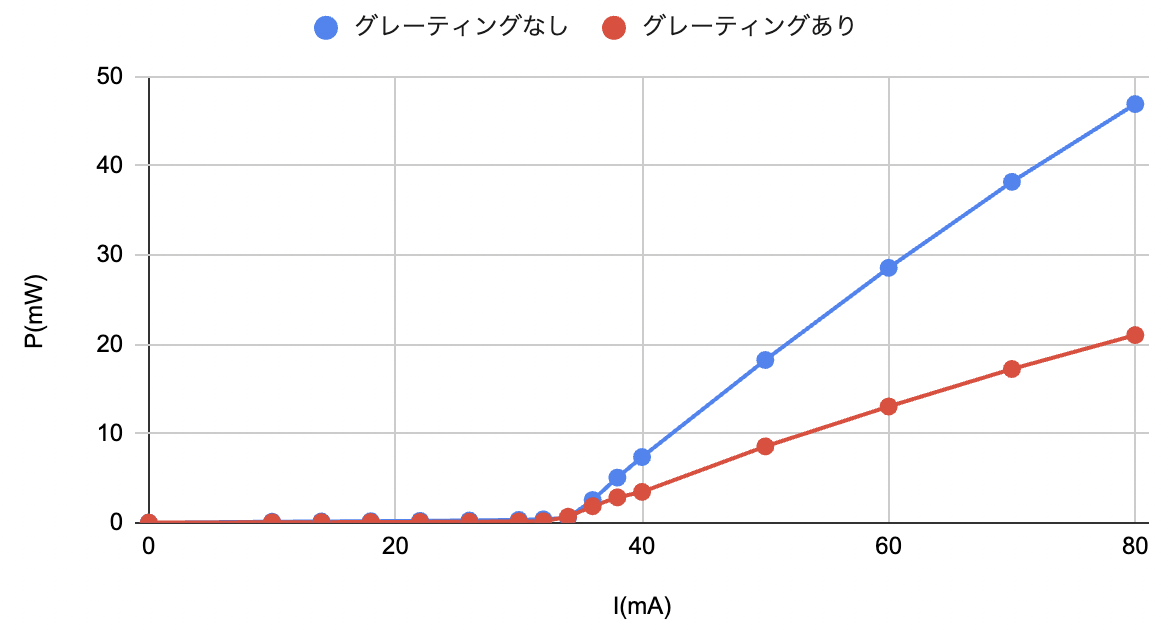
\includegraphics[width=1\textwidth]{images/ld_toptica.png}
\end{minipage}
\begin{minipage}[b]{0.45\linewidth}
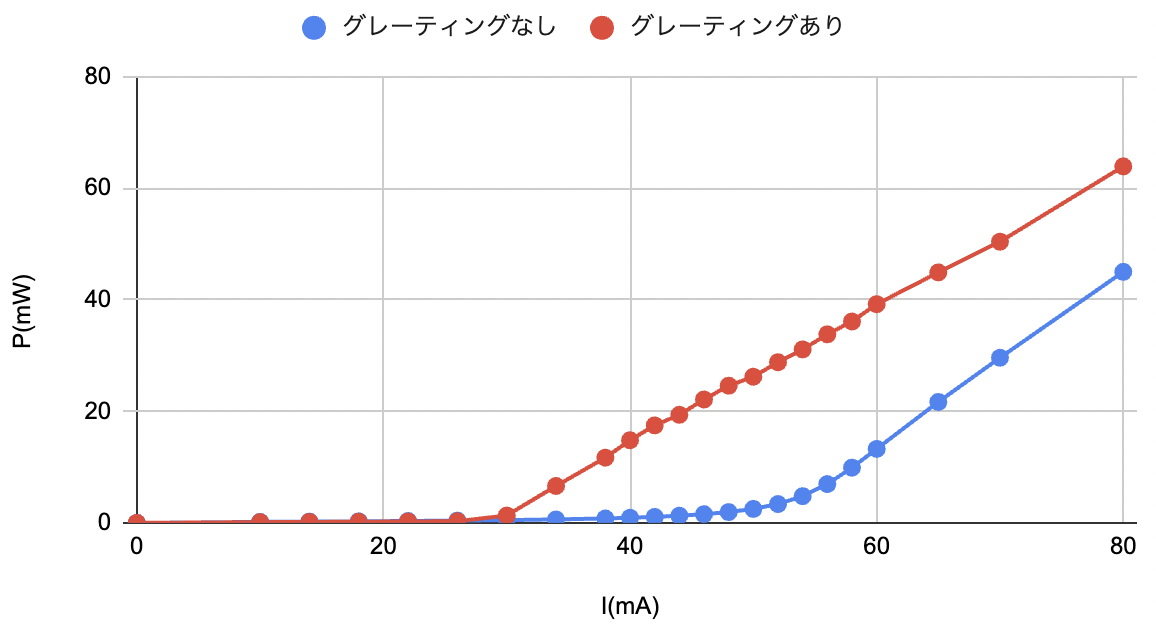
\includegraphics[width=1\textwidth]{images/ld_nicha.png}
\end{minipage}
\caption{\label{fig:ar}グレーティングの有無とP-I特性 (左)ARコート無し (右)ARコートあり}
\end{figure}

\begin{figure}[hbtp]
\centering
\begin{minipage}[b]{0.45\linewidth}
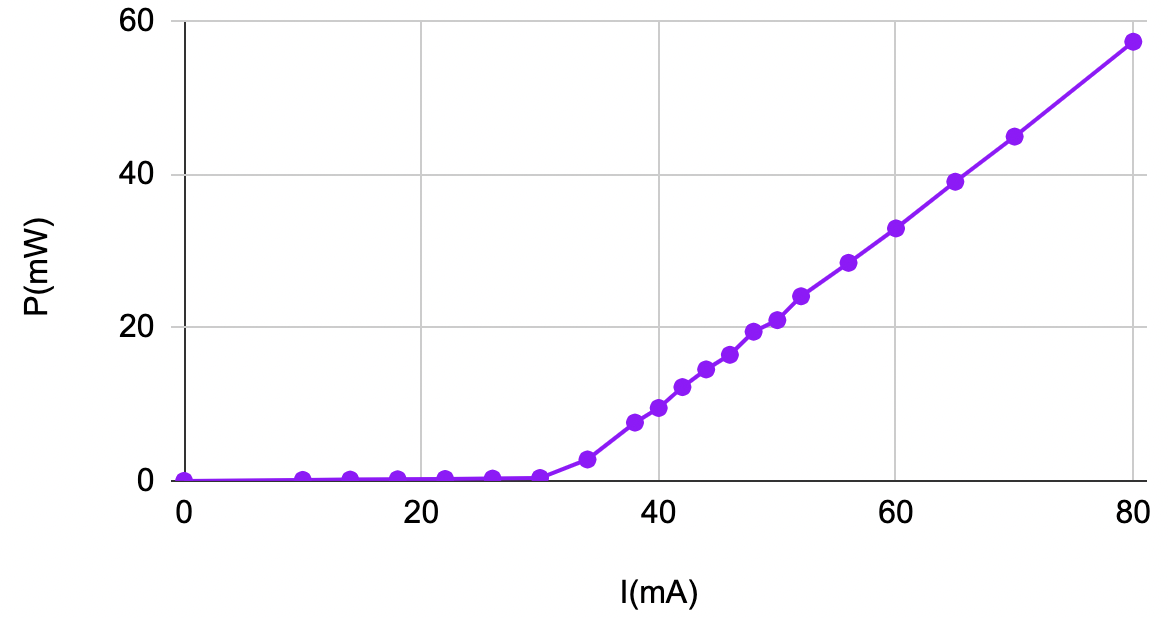
\includegraphics[width=1\textwidth]{images/420-P-I.png}
\end{minipage}
\begin{minipage}[b]{0.45\linewidth}
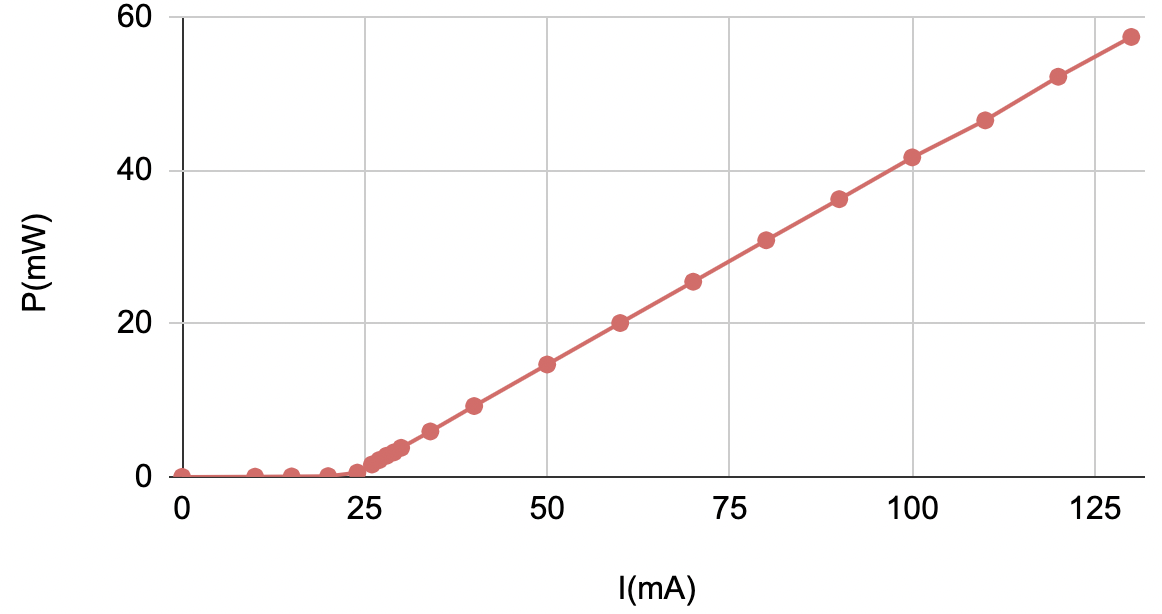
\includegraphics[width=1\textwidth]{images/1024-P-I.png}
\end{minipage}
\caption{\label{fig:p-i}波長調整後のレーザーのP-I特性 (左)ECDL1 (右)ECDL2}
\end{figure}
また、ECDL2については研究室で既に作成されていたものを利用した。グレーティングの角度を調整することで、少なくとも1000nmから1036nmまで周波数を操作できることを確認した。性能評価の基準として、式\ref{rydberg-frequency}よりRbの$6P_{3/2}$から$26D_{5/2}$への励起に必要な波長が約1029.05nm、$6P_{3/2}$から$200D_{5/2}$への励起に必要な波長が約1010.57nmであるので、十分な波長であると言える。レーザー発振に必要な電流は1024nmの時、約26mAであった。こちらのLDは420nmのLDよりスペック上大きな電流に耐えられることができ、電源が最大の130mAの時、レーザーのパワーは57.5mWであった。図\ref{fig:p-i}に各レーザーの入力電流と出力のP-I特性を示す。


\section{ECDL1の周波数安定化}
ECDL1の周波数安定化には、変調移行分光を用いた。光学系の概要は図\ref{fig:mt}に示してある。ECDLから$\lambda / 2$波長板とPBSによって分けてきた光を、さらに$\lambda / 2$波長板とPBSによって強いpump光と弱いprobe光に分けた。pump光はおよそ1mW、probe光はおよそ0.3mW程度のパワーとした。pump光はEOMを通ってPBSで反射し、Rb蒸発セルでprobe光と重ね合わされる。probe光はセルを通過したのち、PBSを透過してそのままPDへと向かう。また、Rb蒸発セルには、温度を調節できるようにヒーターを巻きつけた。
\begin{figure}
\centering
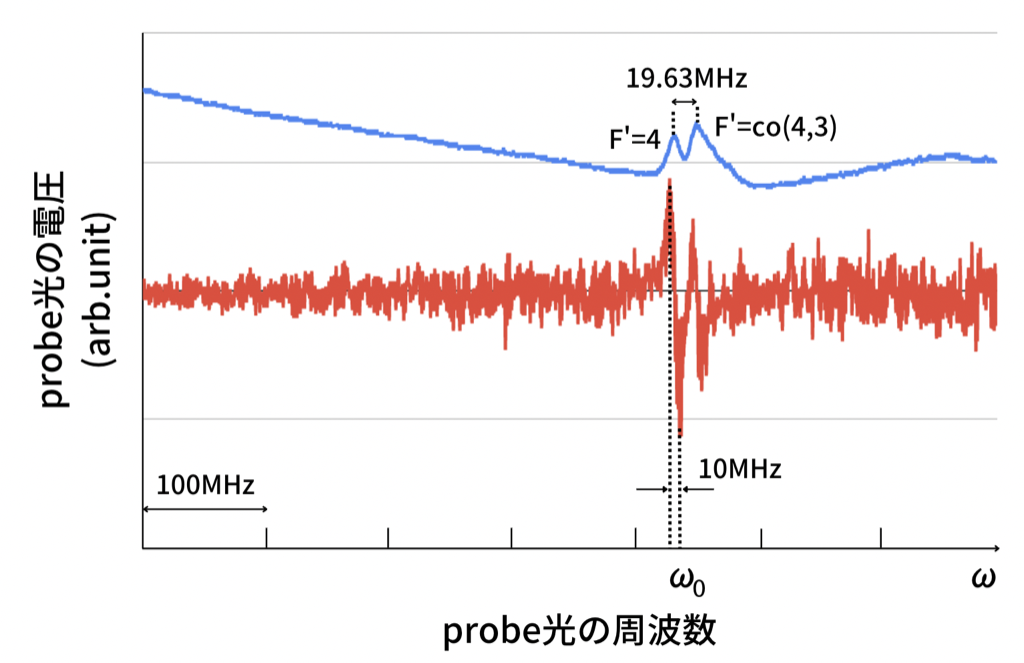
\includegraphics[width=0.8\textwidth]{images/mt85_graph.png}
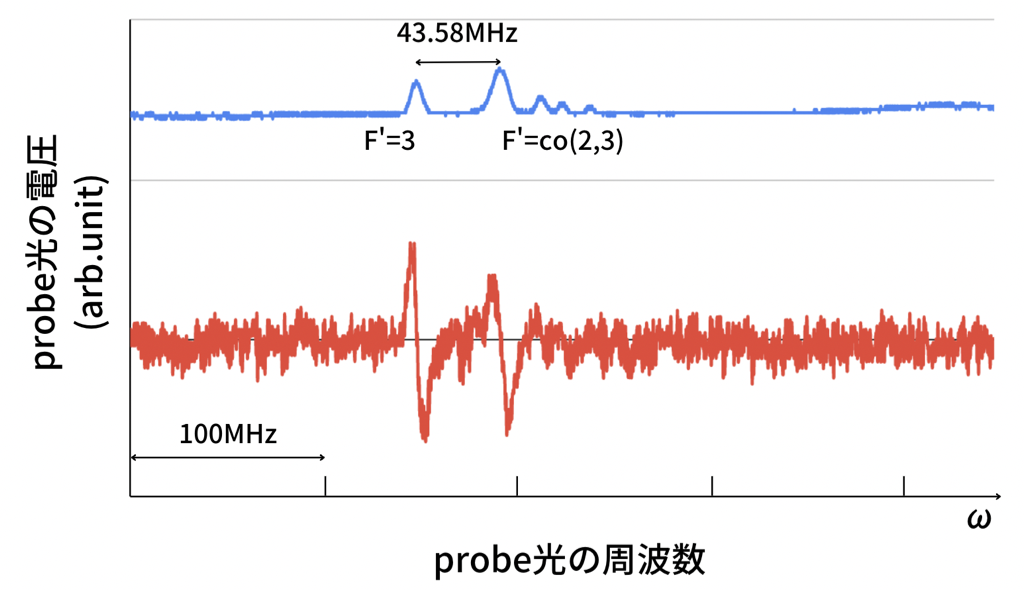
\includegraphics[width=0.8\textwidth]{images/mt87_graph.png}
\caption{\label{fig:mt-graph}飽和吸収と変調移行分光の信号 青色は飽和吸収信号、赤色は変調移行分光の信号。上の図は$^{85}Rb$の$F=3$から$F^{'}=(2,3,4)$の遷移周波数周辺、下の図は$^{87}Rb$の$F=2$から$F^{'}=(1,2,3)$の遷移周波数周辺を観測している。}
\end{figure}
実際にレーザー周波数のロックに用いた信号を図\ref{fig:mt-graph}に示す。青いラインは飽和吸収信号を表しており、上の図は$^{85}Rb$の$F=3$から$F^{'}=(2,3,4)$の遷移に対応するラムディップ、下の図は$^{87}Rb$の$F=2$から$F^{'}=(1,2,3)$の遷移に対応するラムディップが見えている。なお、これらの飽和吸収信号は先行研究\cite{takase-y}\cite{1.6}で得られたものと同様の波形であるため、各ラムディップがどの遷移やクロスオーバーに対応したものかがわかる。また、飽和吸収のラムディップの間隔から、横軸の周波数単位を推定している。超微細構造間の周波数については、\cite{hyperfine}の研究結果から引用した。オシロスコープの横軸の目盛を推定するため、後に出てくるグラフにも同時に観測した飽和吸収分光のスペクトルが頻繁に登場する。

また、赤いラインは変調移行分光の信号であり、共鳴周波数でゼロクロスする勾配の急な信号が取得できている。

図\ref{fig:mt-lock}は、エラー信号をServo回路を通してフィードバックし、実際にレーザー周波数を$^{87}Rb$の$F=2$から$F^{'}=3$の飽和吸収信号にロックした時の様子である。PDで観測されたレーザーの電圧が飽和吸収信号のピークの電圧値に安定化されており、波長計で測定していたレーザーの周波数も713.28180THzにロックされていた。エラー信号の幅は飽和吸収信号の線幅と同じくらいであることからも、レーザー周波数を$\pm 5$MHz程度にロックできていると言える。
\begin{figure}
\centering
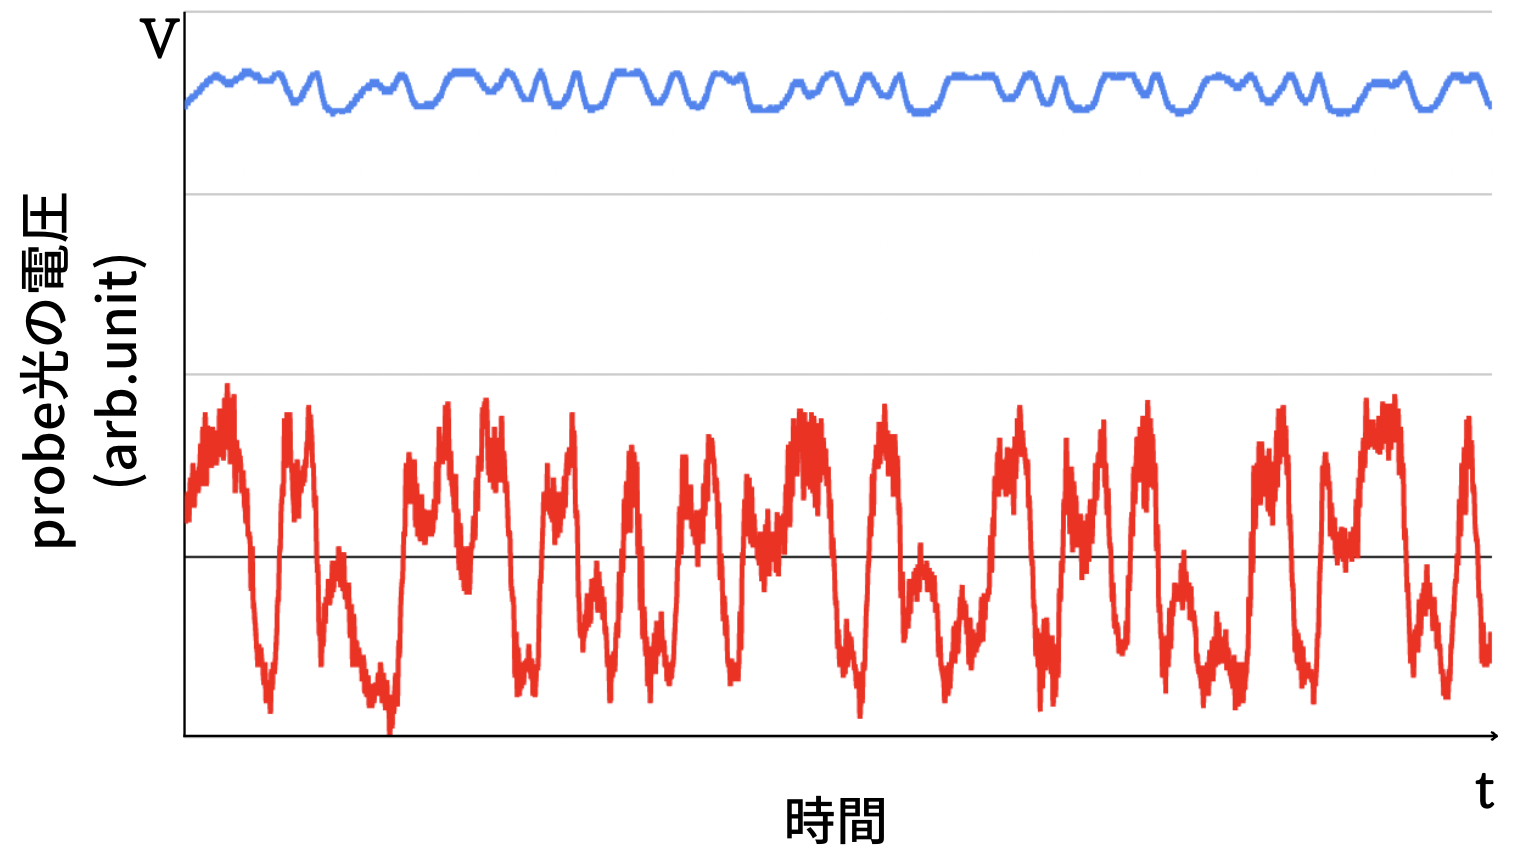
\includegraphics[width=0.7\textwidth]{images/mt_lock.png}
\caption{\label{fig:mt-lock}レーザー周波数をロックしたときの波長計}
\end{figure}

\subsection{Servo回路}

\begin{figure}
\centering
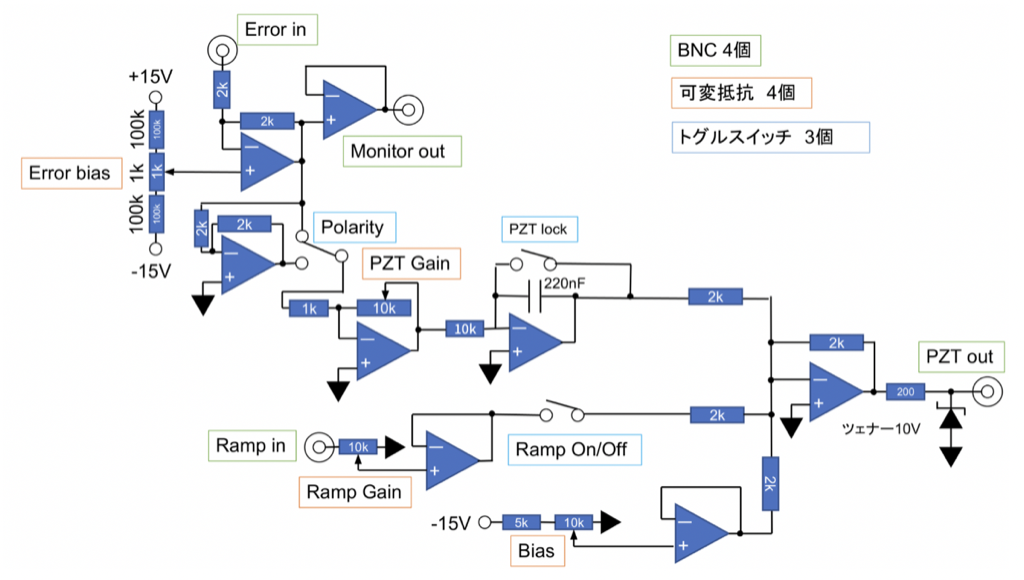
\includegraphics[width=0.8\textwidth]{images/servo.png}
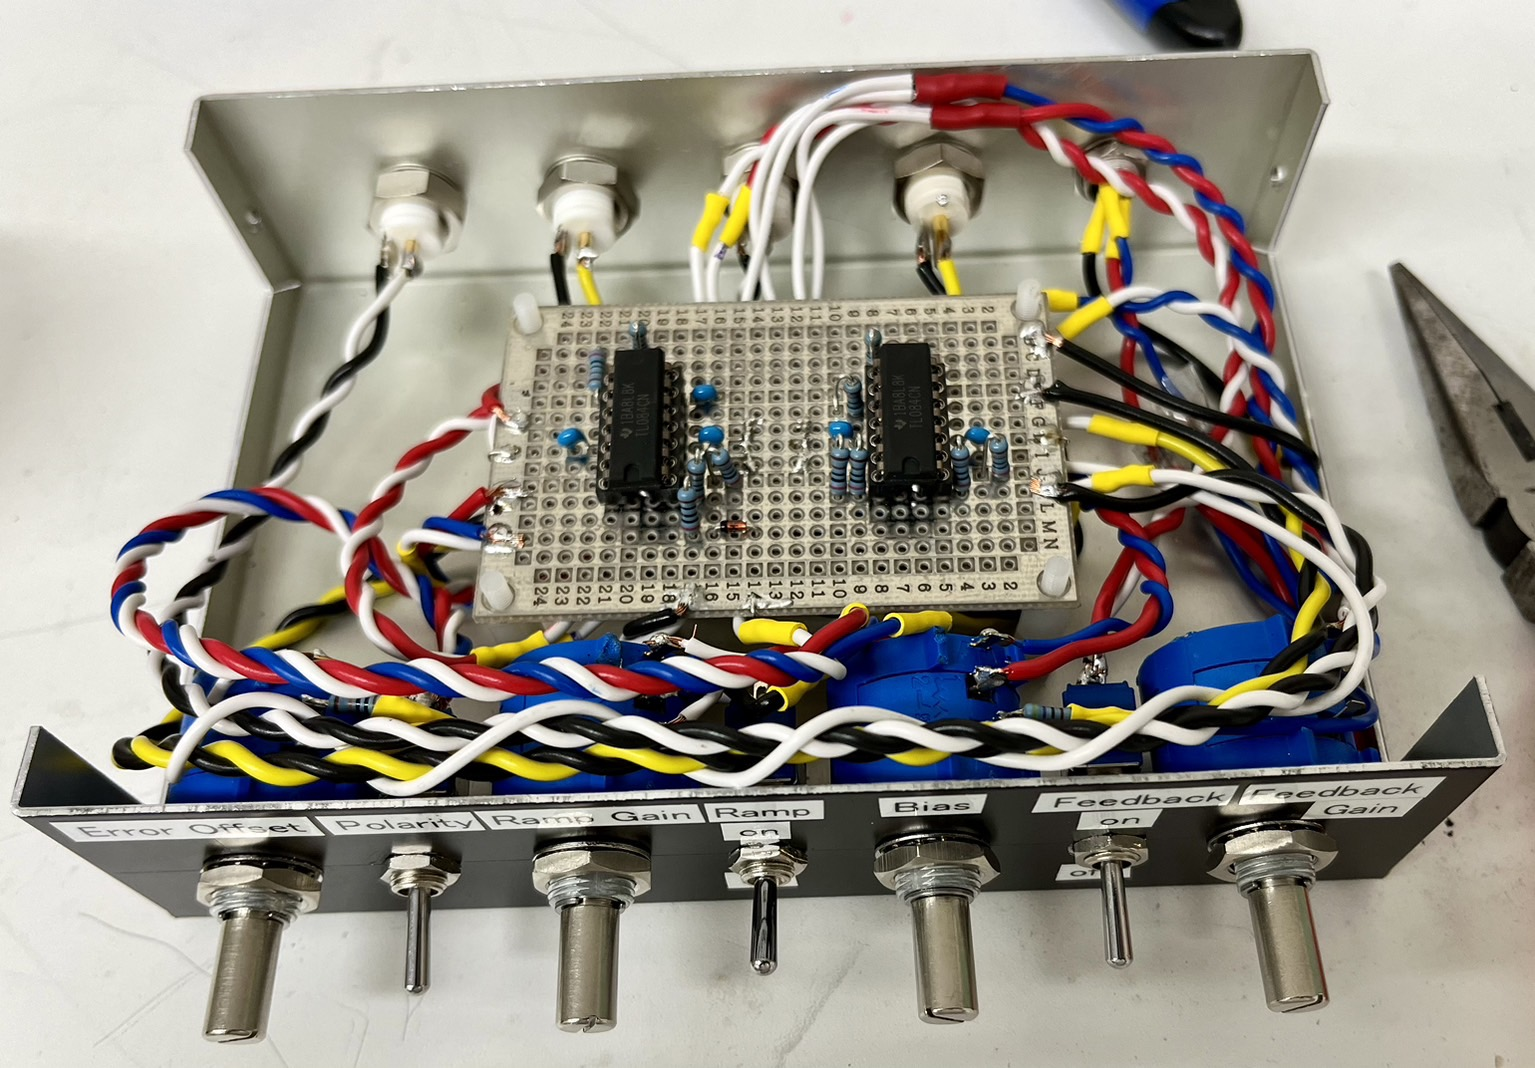
\includegraphics[width=0.8\textwidth]{images/servo_real.jpg}
\caption{\label{fig:servo}上:420nmレーザーのロックに用いたServo回路の回路図 下:実際のServo回路の正面写真}
\end{figure}

実際にECDL1の周波数操作およびエラー信号のフィードバックに用いたServo回路を図\ref{fig:servo}に示した。Biasの可変抵抗を操作することで、PZT素子にかける電圧を連続的に操作することができる。Rampには5.5Vの三角波を入れ、PZT素子を周期的に動かすことでレーザー周波数を振ることができる。この際、可変抵抗によって三角波の振幅を操作、スイッチによってRamp電圧のon/offができる。Error inには変調移行分光などで得られたエラー信号を入れる。Error biasで信号のオフセットを微調整でき、Monitor outで調整後のエラー信号を観測できる。Polarityのスイッチはエラー信号の値を反転させることができる。その後、PZT Gainの可変抵抗によってエラー信号の大きさを調整でき、積分回路はローパスフィルターの役割を果たす。PZT outにてServo回路から出力された信号は、PZT Driverに接続され15倍に増幅されてPZT素子に送られる。この際、PZT Driverの入力電圧を制御するため、10Vのツェナーダイオードが追加されている。


\section{ECDL2の周波数安定化}
ECDL2は$6P_{3/2}$からRyderg準位への励起に使用するが、周波数安定化の参照として使える信号が無く、複数のRydberg準位への励起も予定している。そのため、柔軟にロックする周波数を設定することができる波長計ロックを採用した。波長計ロックとは、レーザーの周波数を波長計で計測し、得られたデジタル信号とプログラムで設定した任意の周波数との誤差を、電圧としてECDLにフィードバックする手法である。ECDL1同様Servo回路を通してフィードバック電圧の大きさを調整し、それをPZT Driverで増幅してPZT素子にフィードバックした。図\ref{fig:wave-lock}にロックした際の周波数と設定値との誤差の時間推移、図\ref{fig:wave-servo}に作成したServo回路の回路図を示す。周波数が、$\pm$ 4MHz程度に安定化されているのが読み取れる。

\begin{figure}[hbtp]
\centering
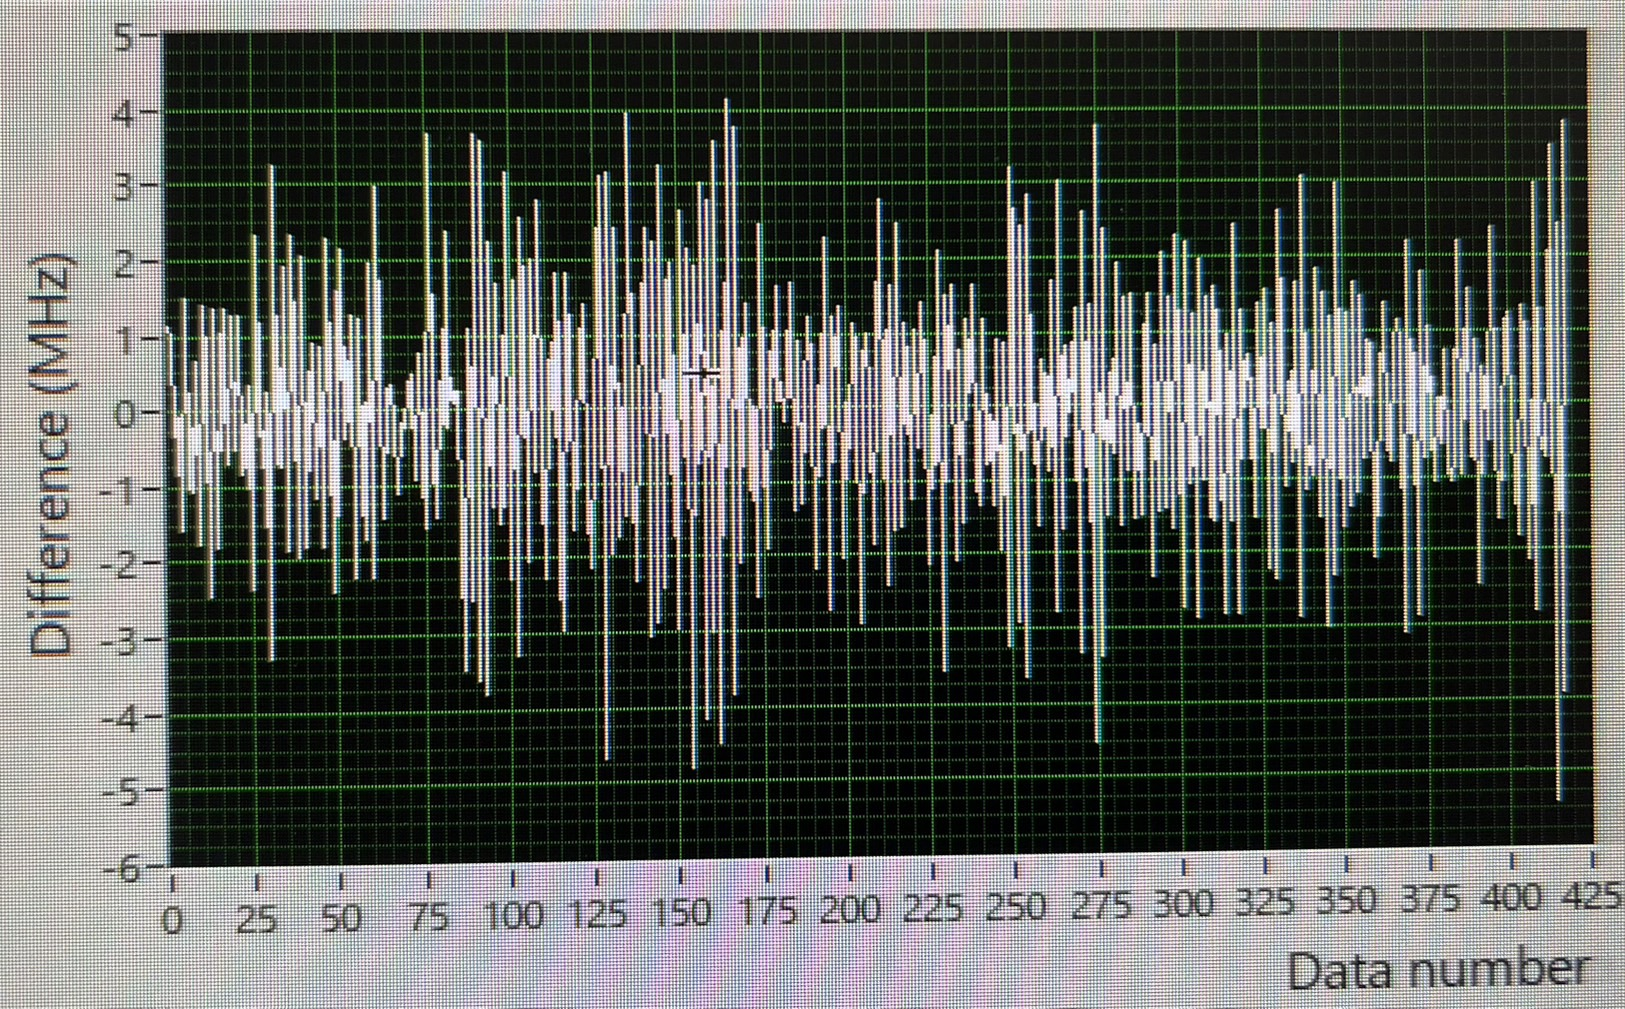
\includegraphics[width=0.8\textwidth]{images/wave_lock.jpg}
\caption{\label{fig:wave-lock}波長計ロックした際の計測周波数と設定値との誤差の時間推移}
\end{figure}

\begin{figure}[hbtp]
\centering
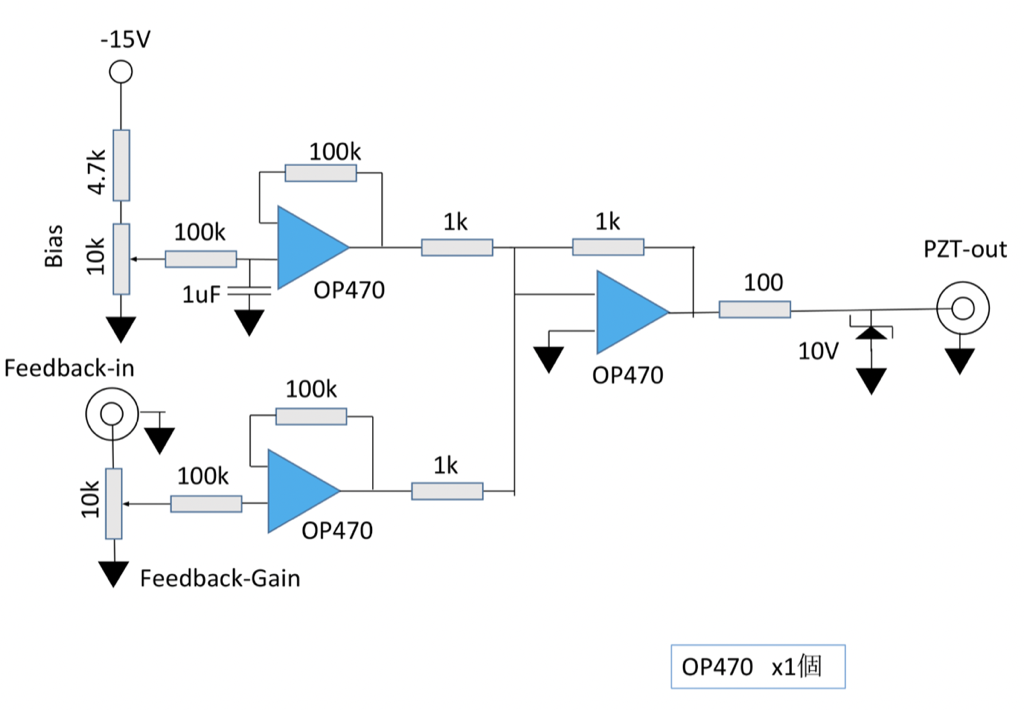
\includegraphics[width=0.8\textwidth]{images/wave_servo.png}
\caption{\label{fig:wave-servo}ECDL2のServo回路}
\end{figure}

\clearpage
\chapter{電磁誘起透明化信号の観測実験}
\section{実験方法}
\begin{figure}
\centering
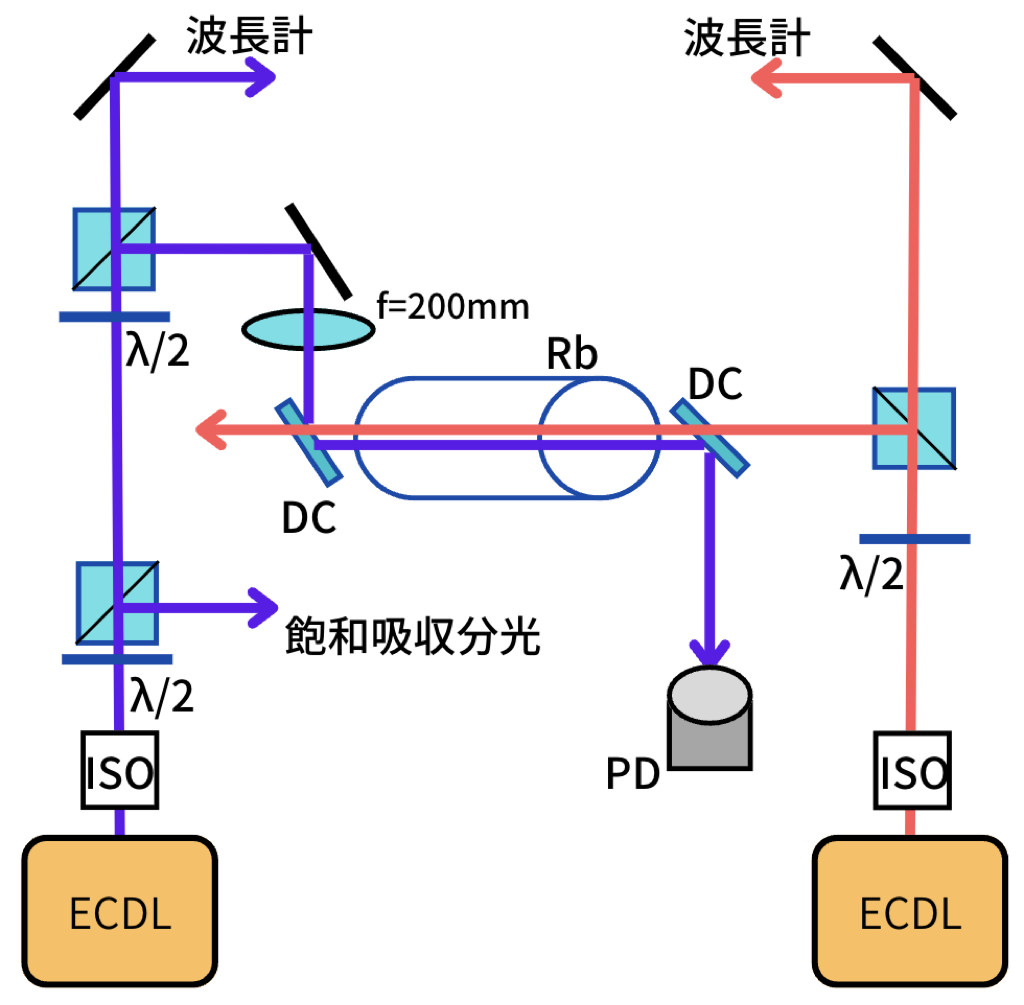
\includegraphics[width=0.6\textwidth]{images/eit.png}
\caption{\label{fig:eit}上:EIT信号観測実験の概要 各レーザーから光を分け、Rb蒸発セル内で重ね合わせ、420nmの光をPDで観測した。なお、各レーザーの手前に設置したアイソレーターや、PBSの前に設置した波長板は省略している。DCはダイクロイックミラー}
\end{figure}
EIT信号を観測するために用いた光学系の概要を図\ref{fig:eit}に示す。各レーザーからPBSで光を分け、Rb蒸発セル内で重ね合わせた。この時、焦点距離200mmのレンズを置くことによってECDL1(=probe光)のレーザー径を小さくし、完全にECDL2(=coupling光)の光に重なるようにしている。レーザー径が小さくなることでprobe光の電場強度は半径の二乗に反比例して大きくなるため、レンズの焦点はセルよりも約8cmほど奥になるような位置に置いている。また、Rb蒸発セルには飽和吸収信号の観測実験と同様に温度を調節するためのヒーターを巻きつけた。実験中のセルの温度は約100℃から120℃で、この範囲においてEIT信号はセルの温度が高いほど強度も大きかった。実験の操作としては、coupling光を計算によって求めた特定の周波数付近に波長計ロックし、ECDL1のPZT素子に三角波電圧をかけることによって周波数を振ったprobe光の電圧をフォトダイオードで観測した。

\section{信号の観測}
遷移双極子モーメント及びラビ周波数は${n^*}^{-3/2}$に比例するため\cite{yuma}、実効主量子数が小さいほどEIT信号のピークの強度は大きくなる。まずはECDL2のスペックで最もピークが見やすいと考えられる$26D_{5/2}$への励起周波数にcoupling光をロックし観測を試みた。EIT信号の観測にはラビ周波数$\Omega_c$が$\Omega_p$に比べて大きいことが重要であるため、coupling光の強度は周波数が合わせられる最大強度とした。(周波数によって、約25mWから35mWの間であった。)

probe光は当初はなるべく小さい20$\mu$W程度の光を入れていたが、いくらcoupling光の周波数を変えてもEIT信号は観測されなかった。その後、probe光を600$\mu$W程度までパワーを上げることによってEIT信号を観測することに成功した。先行研究\cite{optimize}が示すように、probe光が弱すぎてもEIT信号が小さくなり観測できないことがわかった。ただし、パワーを上げるとECDLの発振周波数が共鳴周波数に合わなくなってしまうため、連続的にパワーを上げることが難しく、今回はEITピーク強度の最適化は行っていない。

\begin{figure}[hbtp]
\centering
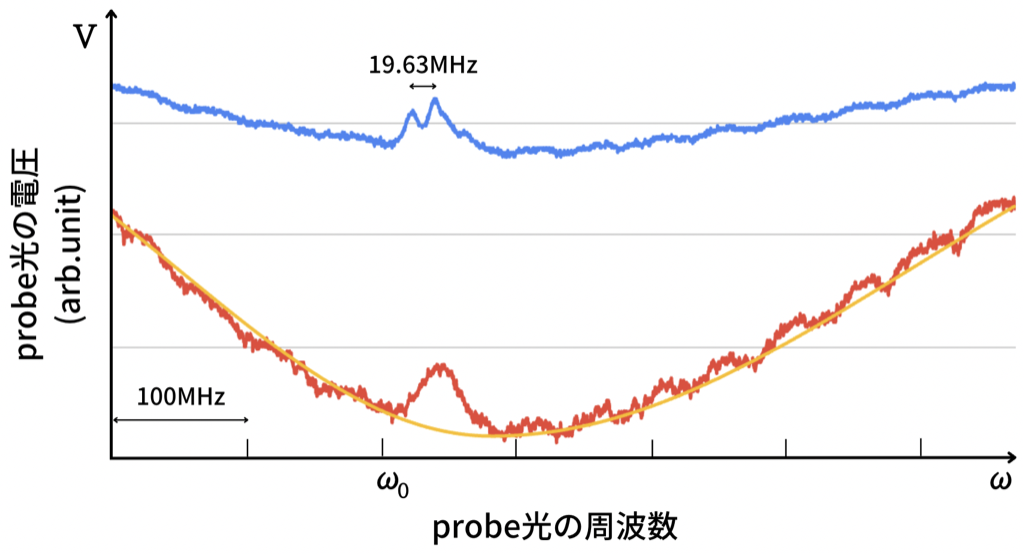
\includegraphics[width=0.7\textwidth]{images/eit26.png}
\caption{\label{fig:eit26}n=26のEIT信号(85Rbの共鳴周波数付近) 青は飽和吸収信号、赤はEIT信号、黄色はEIT信号のドップラー吸収にフィッティングしたガウス関数}
\end{figure}
\begin{figure}[hbtp]
\centering
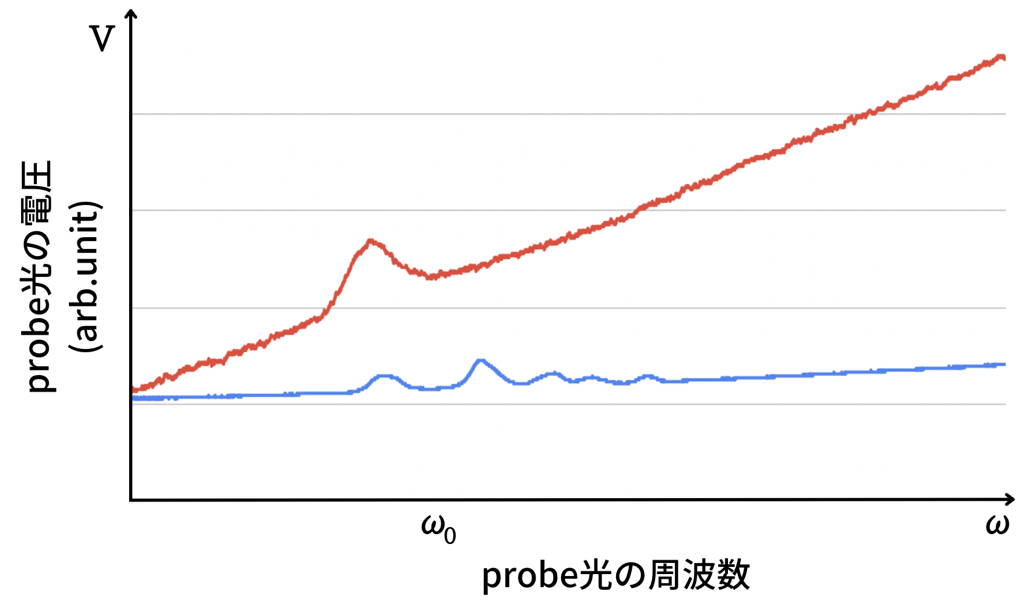
\includegraphics[width=0.7\textwidth]{images/eit87.png}
\caption{\label{fig:eit87}n=26のEIT信号(87Rbの共鳴周波数付近)青は飽和吸収信号、赤はEIT信号}
\end{figure}

\begin{figure}
\centering
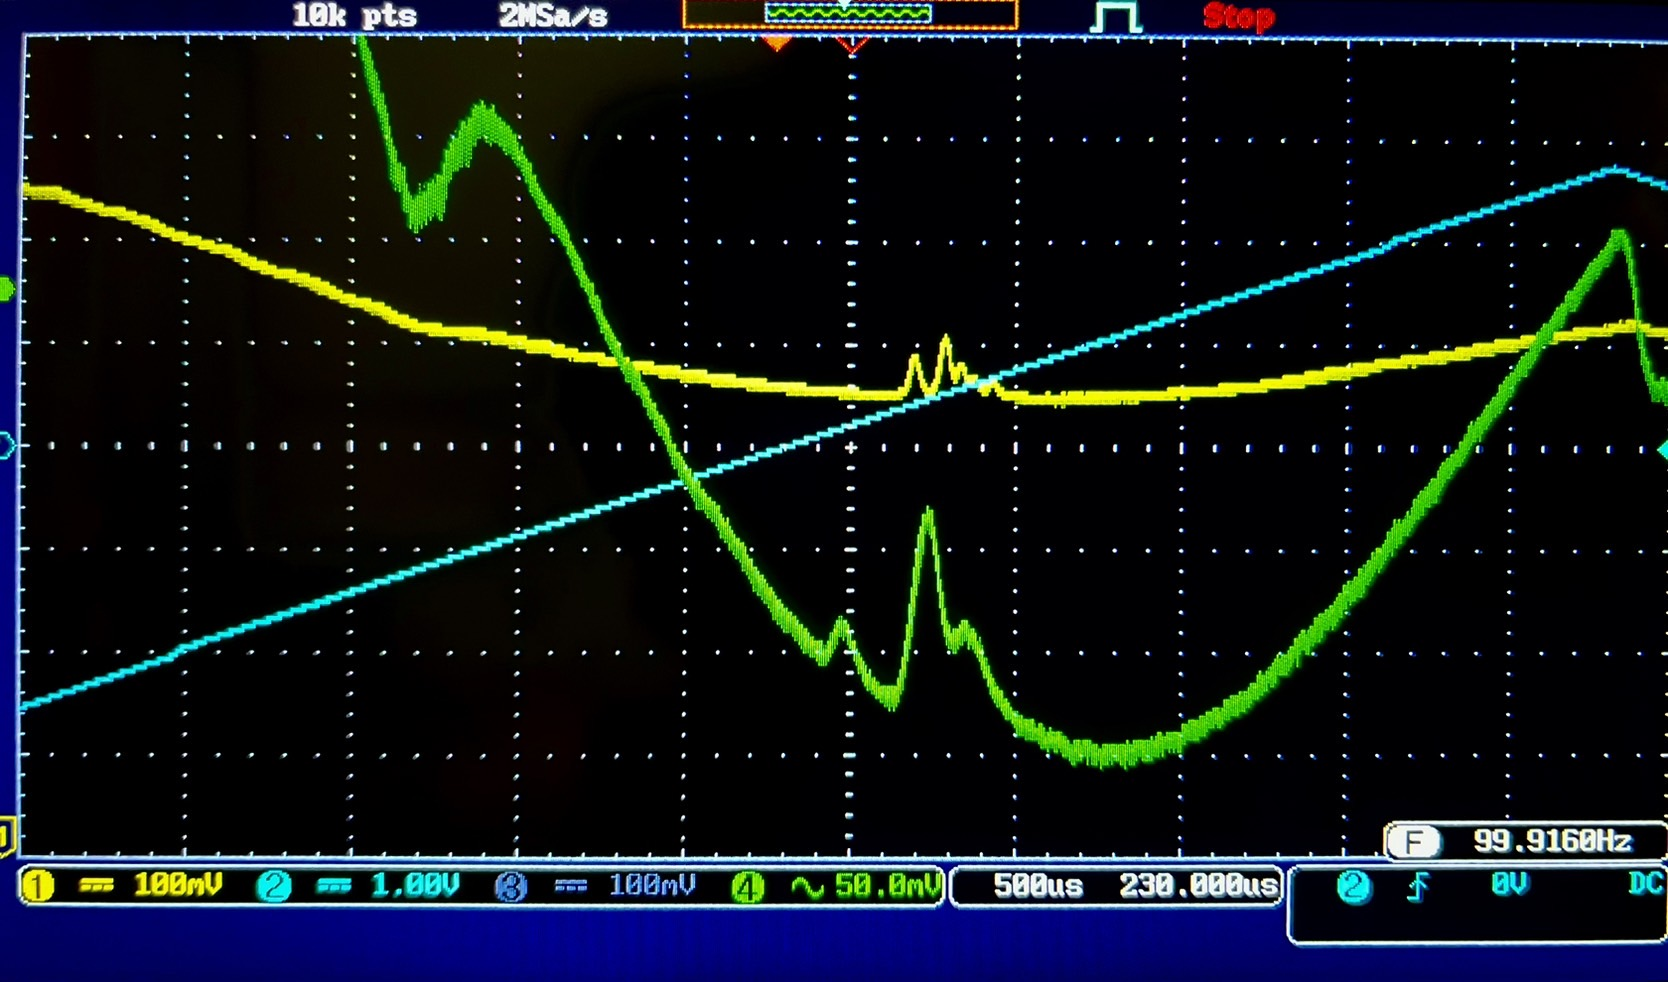
\includegraphics[width=0.7\textwidth]{images/eit_high.jpg}
\caption{\label{fig:eit-high}probe光強度14.5mWの時のオシロスコープ CH1は飽和吸収信号、CH4はEIT信号}
\end{figure}

\begin{table}[hbtp]
  \caption{EIT信号が観測された時のcoupling光の周波数(n=26)}
  \label{table:eit26}
  \centering
  \begin{tabular}{lcr}
    \hline
    coupling光の周波数[THz] & 計算値[THz] & 誤差[THz]  \\
    \hline
    291.3283122  & 291.3288723$\pm 0.0005996$ & -0.00056  \\
    \hline
  \end{tabular}
\end{table}
図\ref{fig:eit26},図\ref{fig:eit87}に観測されたEIT信号を、表\ref{table:eit26}にその時のcoupling光の周波数と\ref{sec:rydberg}の計算によって求めた周波数を示す。EIT信号のディップが、85Rbの$F^{'} = \text{co}(4,3)$の吸収線と同じくらいの周波数で表れている。この時、同じcoupling周波数で、87Rbの$F^{'} = 3$に相当する周波数でもディップが確認された。EIT信号の半値幅は飽和吸収分光のディップから推定するに、$35 \sim 40$MHzである。我々は$6P_{3/2}$を中間準位としているので、$\Gamma_2 = 2\pi \times 1.4$MHzに対し、EIT信号の線幅はおよそ$25\Gamma_2 \sim 28.6\Gamma_2$である。EITの線幅が自然幅よりも太い要因の一つとして考えられるのは、図\ref{fig:absorption}にも示したように$\Omega_c$が$\Gamma_2$に比べて大きいことによるドレスト状態のエネルギー準位のシフトが大きいためと考える。

coupling光の周波数に関しては、計算によって求めた値の中央値より560MHzとかなり離れているが、計算値のエラーバーの範囲内である。560MHzも計算値と離れている要因としては、計算に用いた量子欠損は85Rbの値なのに対し、波数$k_{\text{lim}}$と$k_{6P}$の値は参照した文献\cite{nist}(NIST Atomic Spectra Database Levels Data)が同位体シフトを含んだ値だった可能性がある。また、coupling光を$\pm 100$MHzほど離れたところにロックすると、EIT信号はその分左右に離れた場所に観測された。このことから、電磁誘起透明化は本来の共鳴周波数から100MHz程度離れた場所でもドップラー効果によって観測できると言える。

また、試しにprobe光強度を14.5mWまで上げた時のオシロスコープの様子を図\ref{fig:eit-high}に示す。レンズの位置や温度などを探りながらの観測だったため図\ref{fig:eit26}とパワーの大きさのみの純粋な比較とは言えないが、probe光がcoupling光(25 $\sim 35$mW)と同じオーダーのパワーにも関わらず、はっきりとティップが見えている。線幅に関しては、飽和吸収の$F^{'} = 4$と$F^{'} = \text{co}(4,3)$のディップの間隔が19.63MHzなのを踏まえてグラフのメモリから読み取るに、約25MHzである。さらに、中央の大きなディップの左右に別のディップが現れている。左側のディップは中央のディップから約50MHz、右側のディップは中央のディップから約20MHz離れている。85Rbの$6P_{3/2}$の超微細構造は、$F^{'} = 4$と$F^{'} = 3$の間が39.26MHz、$F^{'} = 3$と$F^{'} = 2$の間が20.667MHzなので\cite{hyperfine}、それぞれ左から$F^{'} = 4,3,2$を中間準位としたRydberg励起のEIT信号の可能性が考えられる。

\section{異なるRydberg準位への励起}
続いて、より主量子数の大きいRydberg準位へ励起した際のEIT信号の観測を試みた。n=26の時の観測結果を踏まえて、\ref{sec:rydberg}節の計算によって求められた各周波数から560MHzを引いた周波数にcoupling光をロックしたところ、図\ref{fig:eitn}に示すような信号が得られた。表\ref{table:eit}は各主量子数に励起した際のcoupling光の周波数である。いずれのグラフでも、n=26の時と同様に85Rbの$F^{'} = \text{co}(4,3)$の吸収線と同じくらいの周波数でEITピークが見られている。なお、n=45に関してはEIT信号が小さく、実際の実験でcoupling光を遮蔽したりしても信号を読み取るのは難しかった。EIT信号の大きさはnが大きくなるほど急激に小さくなっている。一方でEIT信号の線幅に関しては、n=30とn=40のグラフを比較しても、少なくとも数十MHzといった読み取れるほどの変化はないと言える。$\Omega_c$は${n^*}^{-3/2}$に比例するので、図\ref{fig:absorption}によれば$\Omega_c$が小さくなるほどEITピークの線幅も狭くなっていくはずであるが、今回の実験ではそのような傾向は見られなかった。
\begin{table}[hbtp]
  \caption{EIT信号が観測された時のcoupling光の周波数}
  \label{table:eit}
  \centering
  \begin{tabular}{lcr}
    \hline
    主量子数n  & ロック周波数[THz]  \\
    \hline
    30  & 292.7338158 \\
    35  & 293.8359072 \\
    40  & 294.5387450 \\
    45  & 295.0142370 \\
    \hline
  \end{tabular}
\end{table}

\begin{figure}[hbtp]
\centering
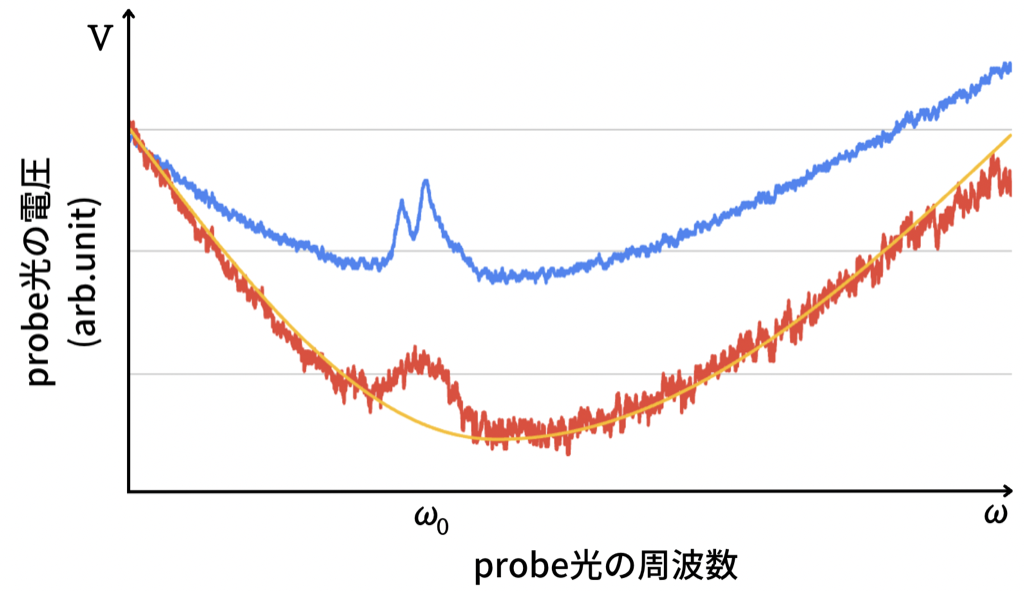
\includegraphics[width=0.6\textwidth]{images/eit30.png}
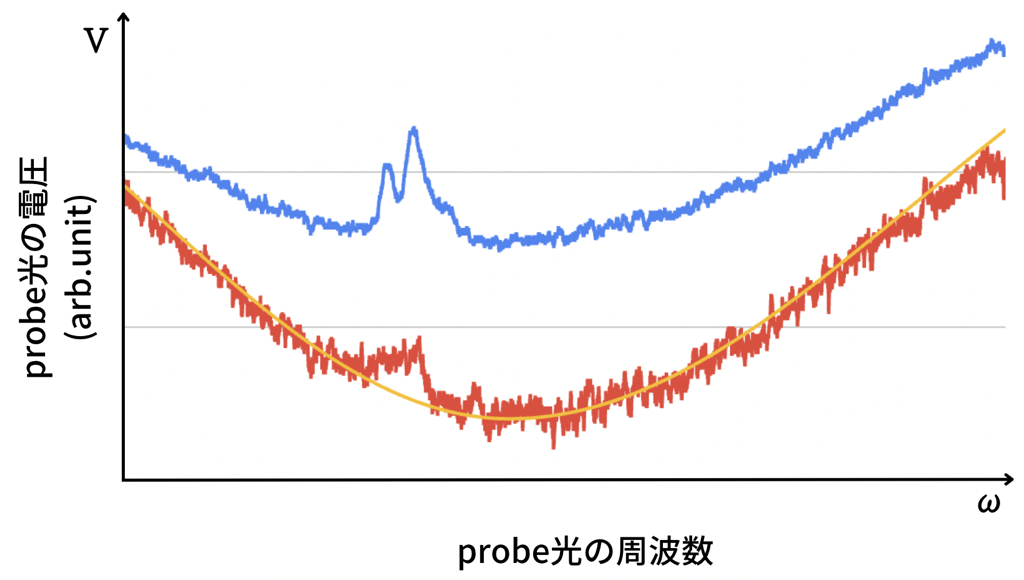
\includegraphics[width=0.6\textwidth]{images/eit35.png}
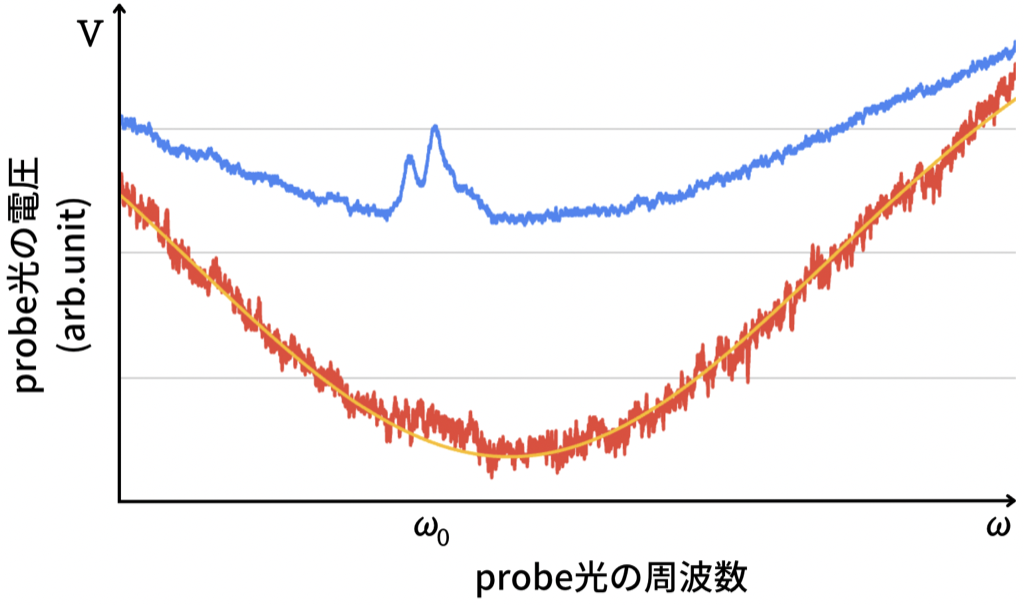
\includegraphics[width=0.6\textwidth]{images/eit40.png}
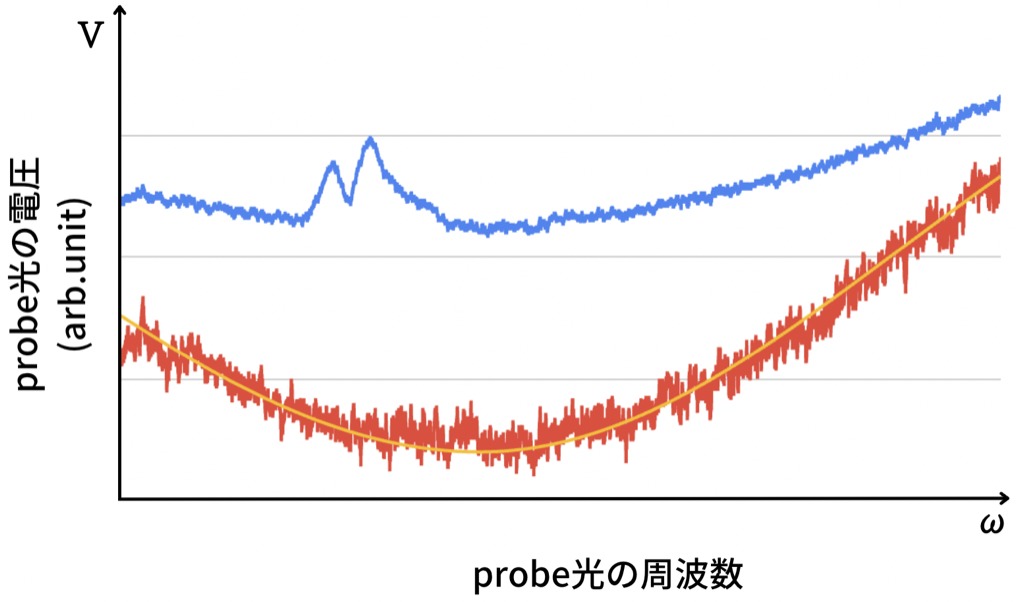
\includegraphics[width=0.6\textwidth]{images/eit45.png}
\caption{\label{fig:eitn}上から順番に、飽和吸収信号とn=30,35,40,45のEIT信号}
\end{figure}

\clearpage
\chapter{まとめ}
本研究では、field ionizationを行うためのRydberg励起用レーザーシステムの開発を目的とし、レーザーの開発からRydberg励起が成功しているかを確認するための電磁誘起透明化信号の観測までを行った。レーザーには、ARコート付きのLD素子を利用した外部共振器型半導体レーザーを作成した。ECDL1はRbの基底状態から$6P_{3/2}$への励起数波数、ECDL2は$6P_{3/2}$から$26D_{5/2}$以上のRydberg準位への励起周波数に対応していることを確認した。ECDL1の周波数安定化には変調移行分光法を用いて、周波数を$\pm5$MHz以内に安定化することができた。ECDL2の周波数安定化には波長系ロックを用いて、周波数を$\pm4$MHz以内に安定化することができた。電磁誘起透明化信号は、$26D_{5/2}$から$40D_{5/2}$までの観測に成功した。周波数が大きくなると信号強度が急激に小さくなるため、それ以上の主量子数のEIT信号を観測することはできなかったが、Rydberg励起に必要なcoupling光の周波数を少なくともレーザーの線幅である$\pm5$MHz以内で精密に計算できるようになったため、今後のEIT信号の観測が格段に簡単になった。

一方で、冒頭で述べたようにfield ionizationを行うには、100V/cmの電場を用意しても$n^*=$42.04482のRydberg原子が必要である。したがって今後の展望としては、よりEIT信号の強度を高めるための実験系の改良や最適化が挙げられる。probe光の強度に関しては、0.6mWと14.5mWといった非常に離れた値での観測しか行っていないため、セルの温度も含めまだまだ最適化の余地があるといえる。また、copuling光をテーパードアンプなどで増幅したり、アイソレーターをより透過率の高いものに変更したりすることで、coupling光の電場強度が上がり、ラビ周波数$\Omega_c$を大きくすることができる。これらの改良を加えることで、field ionizationに十分な主量子数のRydberg状態励起用レーザーが用意できると考える。




\bibliographystyle{alpha}
\begin{thebibliography}{99}
\bibitem{bose}M. H. Anderson et al., Science 269, 198(1995)
\bibitem{fesh}S. Inouye, M. R. Andrews, J. Stenger, H.-J. Miesner, D. M. Stamper-Kurn, and W. Ketterle. Observation of Feshbach resonances in a Bose-Einstein condensate. Nature, 392, pp. 151 – 154, (1998)
\bibitem{efimov}Greene, C. H., Giannakeas, P. and Pérez-Ríos, J. Universal few-body physics and cluster formation. Rev. Mod. Phys. 89, 035006 (2017)
\bibitem{ion-rydberg}Nicolas Zuber, Viraatt S. V. Anasuri, Moritz Berngruber, Yi-Quan Zou, Florian Meinert, Robert Löw and Tilman Pfau "Observation of a molecular bond between ions and Rydberg atoms"  Nature, 605, pp. 453 – 456, (2022)
\bibitem{kobayashi}Jun Kobayashi et al., Nature Comn 10, 3771
\bibitem{okuda}奥田泰崇 「共振器増幅された 3 次元光格子中でのレーザー冷却実験」 北海道大学 2022
\bibitem{rucas}Rucas beguin "Measurement of the van der Waals interaction between two Rydberg atoms" Appendix B, University of Basel 2013
\bibitem{rydberg}T.Gallagher "Rydberg Atoms" Cambridge University Press 2005.
\bibitem{yuma}中村 勇真 「単一イッテルビウム原子を用いた量子計算に向けた光ピンセットアレイシステムの開発とリドベルグ分光」 京都大学大学院 2022
\bibitem{yamamotomasashi} 陳 軍・山本将史 『らくらく図解 光とレーザー』 オーム社 2006
\bibitem{suzuki}鈴木 皓博・井上 慎「光会合用レーザーシステムの開発」 東京大学 2013
\bibitem{foot}C. J. Foot: ”Atomic Physics”, OXFORD UNIVERSITY PRESS (2005)
\bibitem{eit-pertubation}林 暢仁 「ラダー型及び Λ 型 3 準位系における量子干渉効果」 熊本大学大学院 (2011)
\bibitem{eit-absorption}Sumanta Khan, Vineet Bharti, Vasant Natarajan ”Role of dressed-state interference in electromagnetically induced transparency”, Indian Institute of Science (2016)
\bibitem{mt}D. J. McCarron, S. A. King and S. L. Cornish "Modulation transfer spectroscopy in atomic
\bibitem{mt2}池田 幸平 「通信波長帯周波数安定化レーザーと天文コムへの応用」 横浜国立大学大学院 2019
\bibitem{four-wave}矢島 達夫 「非線形光学の基礎II:2次と3次の現象」日本大学 1998
\bibitem{nagaoka-yosuke}長岡 洋介 物理入門コース4 電磁気学$\mathrm{I}\hspace{-1.2pt}\mathrm{I}$ 変動する電磁場 10章
\bibitem{optimize}HSUAN-JUI SU, JIA-YOU LIOU, I-CHUN LIN, AND YI-HSIN CHEN "Optimizing the Rydberg EIT spectrum in a thermal vapor" Vol. 30, No. 2/17 Jan 2022/ Optics Express 1499
\bibitem{takase-y}高瀬 直美 「Rydberg励起用周波数安定化波長420nm半導体レーザーの開発」 電気通信大学 2019
\bibitem{hyperfine}"Hyperfine Structure Measurements of the 85Rb and 87Rb 6P3/2 State" IEEE International Frequency Control Symposium (2019)
\bibitem{1.6}Krishnapriya Subramonian Rajasree, Kristoffer Karlsson, Tridib Ray, and Síle Nic Chormaic "1.6GHz Frequency Scanning of a 482 nm Laser Stabilized Using Electromagnetically Induced Transparency" IEEE PHOTONICS TECHNOLOGY LETTERS, VOL.33, NO.15, AUGUST 1, 2021
\bibitem{quantum-defect}Wenhui Li, I. Mourachko, M. W. Noel, and T. F. Gallagher "Millimeter-wave spectroscopy of cold Rb Rydberg atoms in a magneto-optical trap: Quantum defects of the ns, np, and nd series" University of Virginia, Bryn Mawr College 2003

Quantum defects of the ns, np, and nd series
\bibitem{nist}NIST Atomic Spectra Database Levels Data
\end{thebibliography}
\end{document}

% ダークステート
% \begin{align}
% \psi_{\text{+}} = \frac{1}{\sqrt{2}}\left( |e\rangle + \frac{\Omega_p}{\Omega}|g\rangle + \frac{\Omega_c}{\Omega}|r\rangle  \right) \\
% \psi_{0} = \frac{\Omega_c}{\Omega} |g\rangle - \frac{\Omega_p}{\Omega} |r\rangle\\
% \psi_{\text{-}} = \frac{1}{\sqrt{2}}\left( |e\rangle - \frac{\Omega_p}{\Omega}|g\rangle - \frac{\Omega_c}{\Omega}|r\rangle  \right)
% \end{align}
% $\omega_c$

sips -Z 1024 *.png